%#!platex ./report.tex

 \section{Ka$B%A%c%M%k$rMQ$$$?>l9g$N7k2L(B}
   $B?^(B\ref{Ka_Result1}, $B?^(B\ref{Ka_Result2}$B$K(BKa$B%A%c%M%k$rF3F~$7$?:]$N7k2L$r<($9(B.
   $B?^Cf$N(BGausian$B$O%3%s%@%/%?%s%9J,I[MM<0$K(B
   $B%,%&%9J,I[$rMQ$$$F$*$j(B, Liner$B$O@~7AJ,I[$rMQ$$$?>l9g$N7k2L$G$"$k(B.
   $B$^$?(B-reduced$B$O$=$l$>$l$N%3%s%@%/%?%s%9J,I[MM<0$G(B, $B8DBNI>2A$K%3%s%@%/%?%s%9NL$X$N9MN8(B
   $B$rF3F~$7$?>l9g$N7k2L$G$"$k(B. \\
   $B%0%i%U>eIt$N5-9f$O3F(B${\Delta}t$$B$K$*$$$F(B, $B%&%'%k%A$N(Bt$B8!Dj(B($\alpha = 0.05$)
   $B$r9T$$M-0U:9$,$_$i$l$?$3$H$r(B
   $B<($7$F$$$k(B. $B5-9f(B($\star$)$B$O(BGausian$B$H(BLiner$B$N7k2L$rHf3S$7$F$$$k(B. 
   $B5-9f(B($\#$)$B$O(BGausian$B$H(Breduced-Gausian, Liner$B$H(Breduced-Liner$B$NAH$G8!Dj$r9T$C$?7k2L$G$"$k(B.
   $B$^$?NP?'$N5-9f(B($+$)$B$O(Breduced-Gausian$B$H(Breduced-Liner$B$NAH$G8!Dj$r9T$C$?7k2L$r<($7$F$$$k(B. 
   \vspace{-0.5cm}
     \begin{figure}[H]
       \begin{subfigure}{0.5\columnwidth}
         \centering
         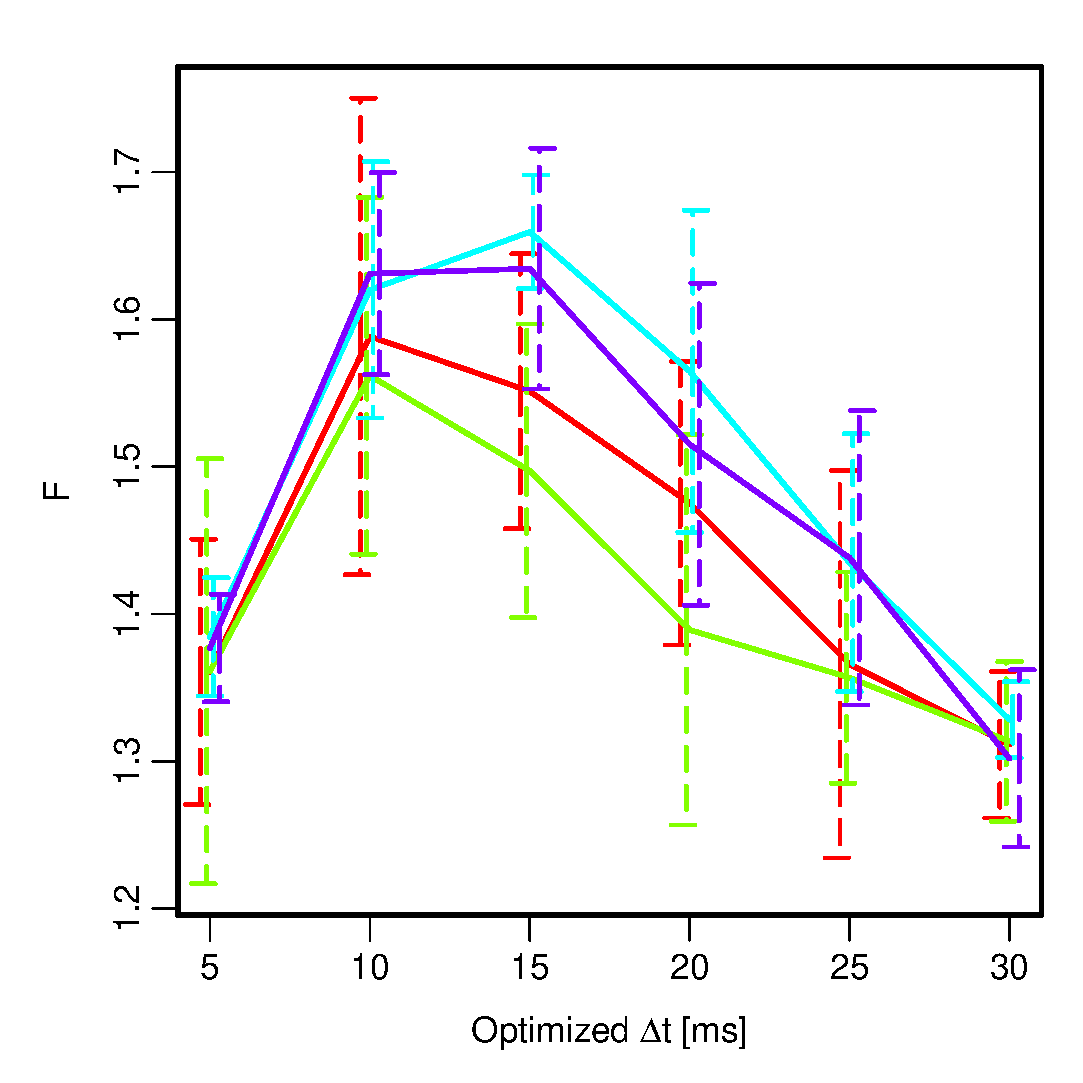
\includegraphics[width=0.8\columnwidth]{./Images_Result/k_test_F.eps}
         \caption{$F$}
         \label{k_F}
       \end{subfigure}
       \begin{subfigure}{0.5\columnwidth}
         \centering
         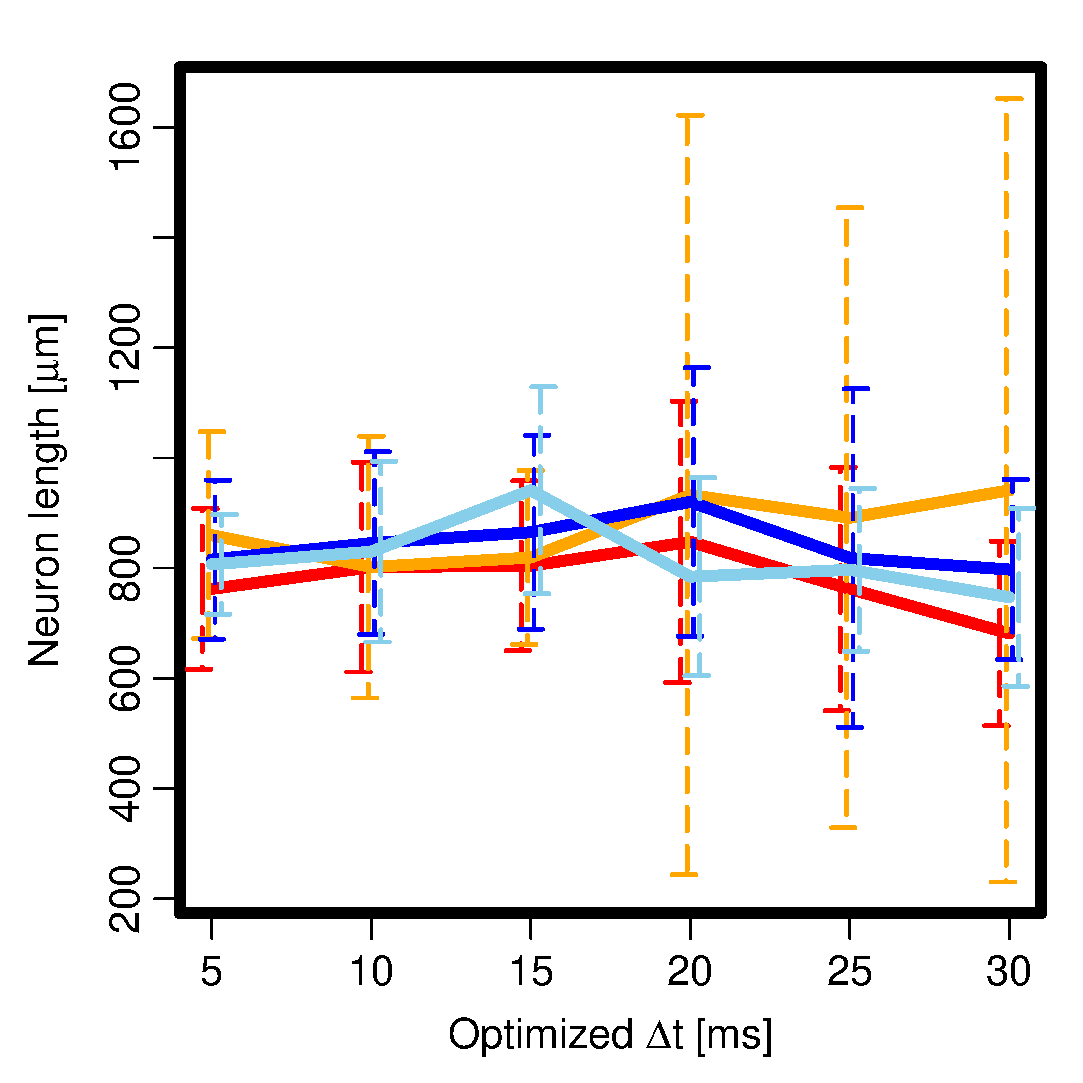
\includegraphics[width=0.8\columnwidth]{./Images_Result/k_test_TREE_length.eps} 
         \caption{$BD9$5(B}
         \label{k_TREE_length}
       \end{subfigure}

       \begin{subfigure}{0.5\columnwidth}
         \centering
         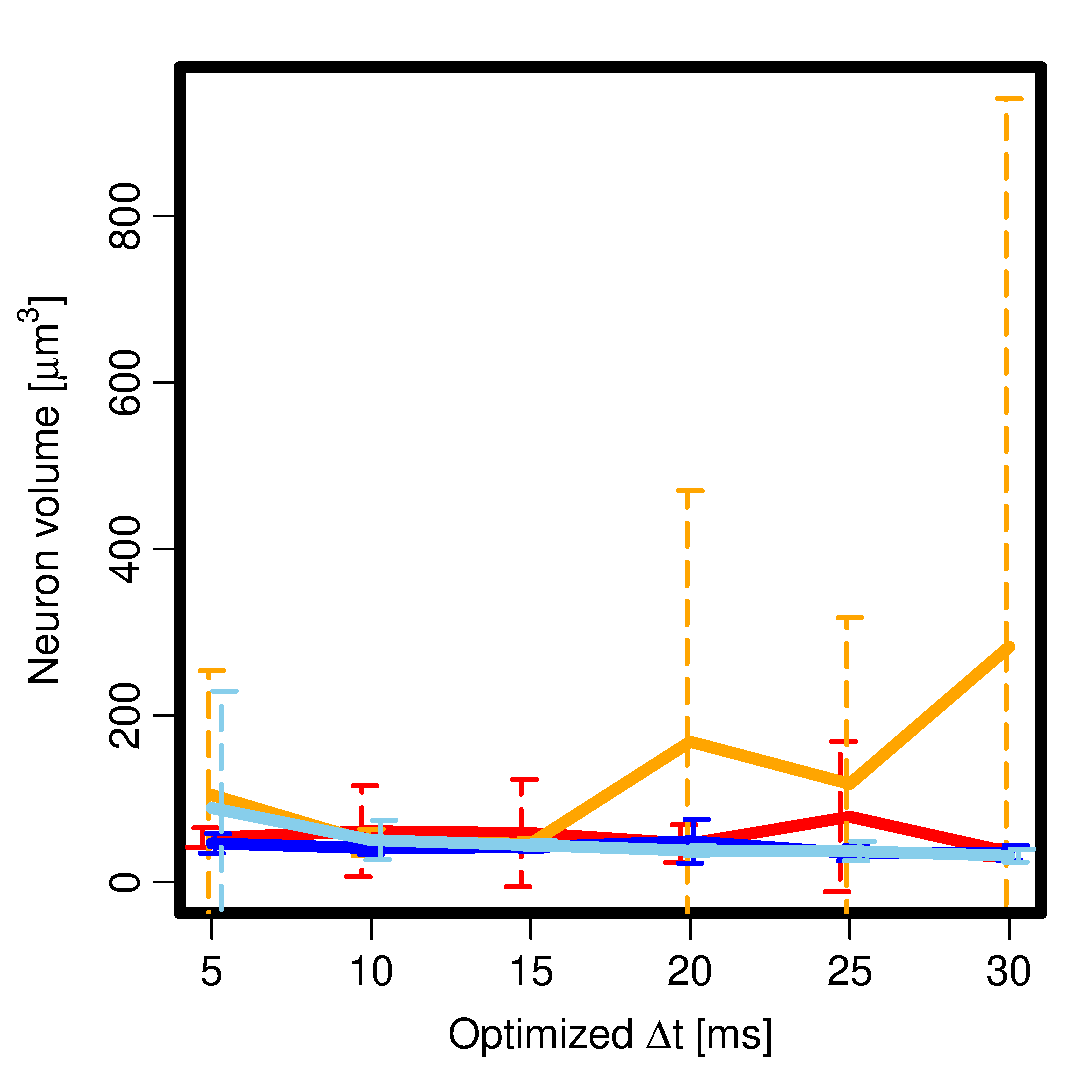
\includegraphics[width=0.8\columnwidth]{./Images_Result/k_test_TREE_volume.eps}
         \caption{$BBN@Q(B}
         \label{k_TREE_volume}
       \end{subfigure}
       \begin{subfigure}{0.5\columnwidth}
         \centering
         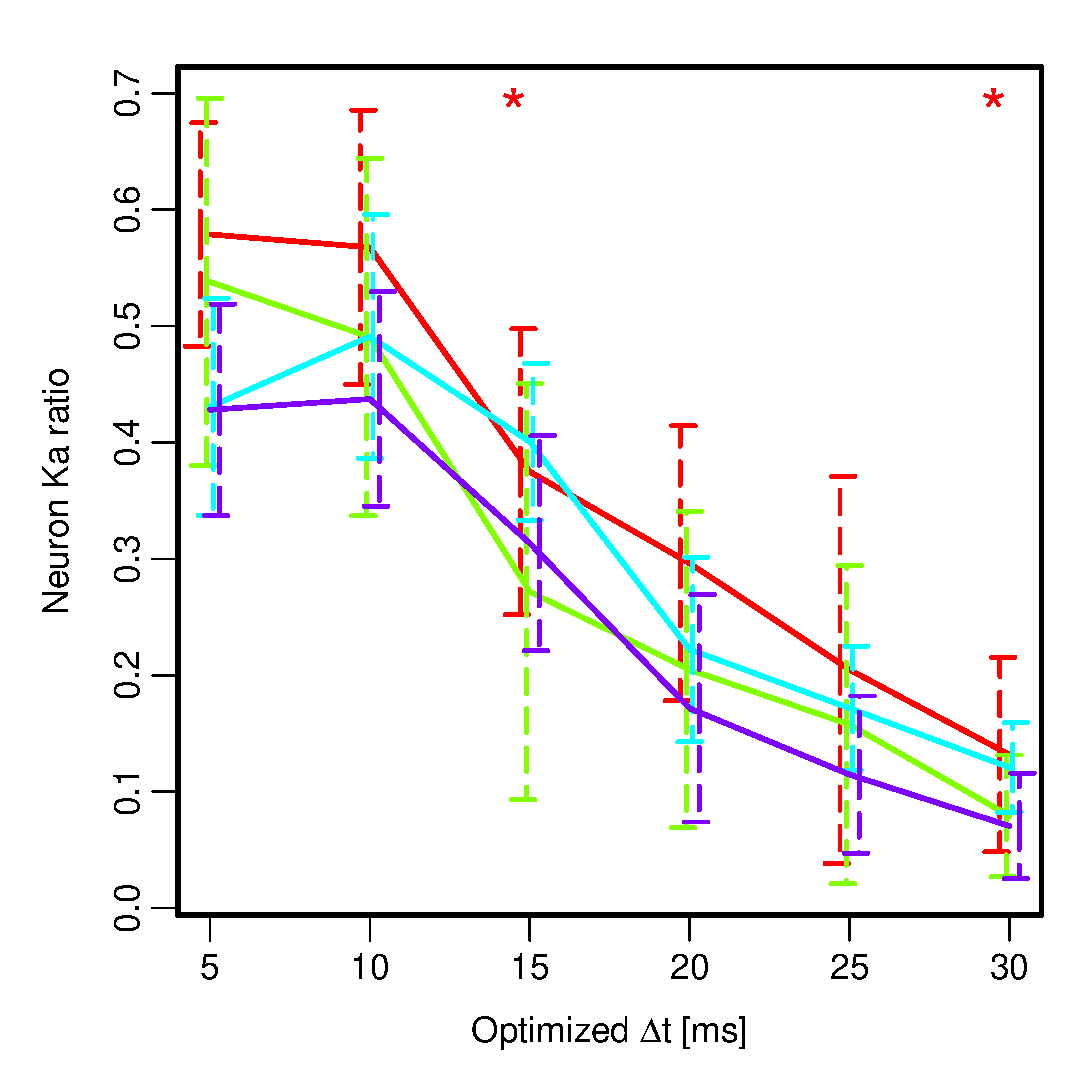
\includegraphics[width=0.8\columnwidth]{./Images_Result/k_test_TREE_K_ratio.eps}
         \caption{Ka$B%3%s%@%/%?%s%94^M-N((B}
         \label{k_TREE_K_ratio}
       \end{subfigure}

       \begin{subfigure}{0.5\columnwidth}
         \centering
         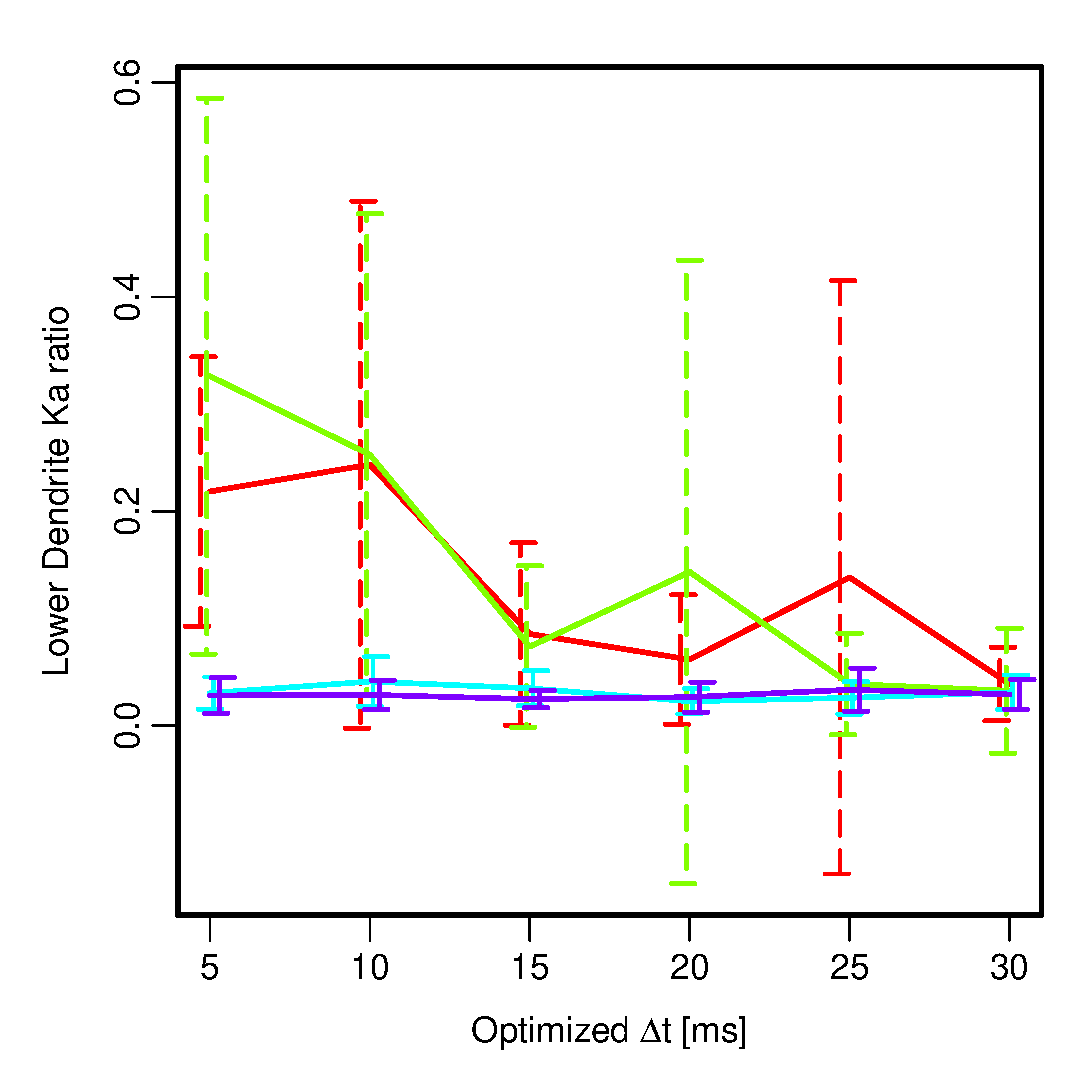
\includegraphics[width=0.8\columnwidth]{./Images_Result/k_test_Lower_K_ratio.eps}
         \caption{Lower Dendrite$B$N(BKa$B%3%s%@%/%?%s%94^M-N((B}
         \label{k_lower_k_ratio}
       \end{subfigure}
       \begin{subfigure}{0.5\columnwidth}
         \centering
         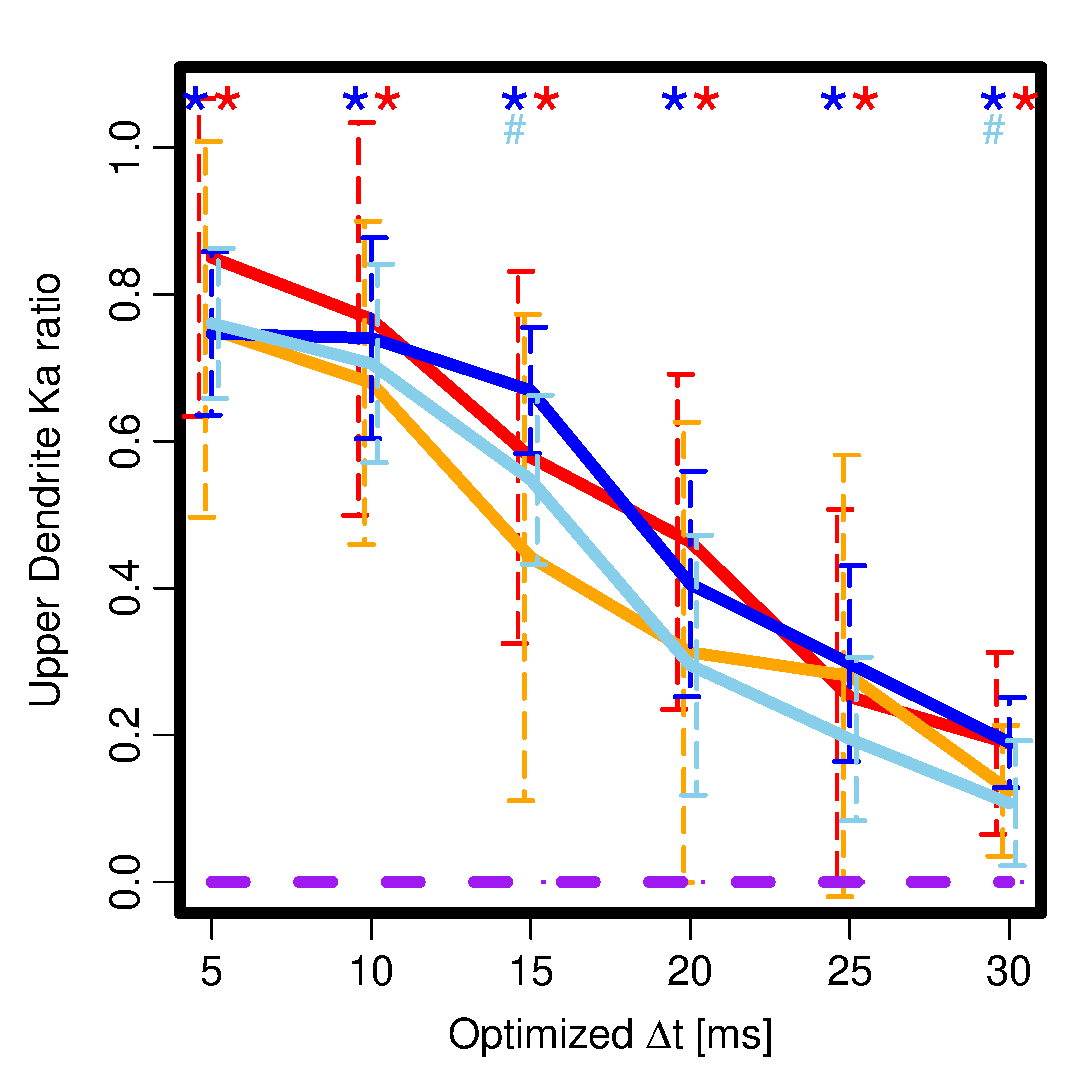
\includegraphics[width=0.8\columnwidth]{./Images_Result/k_test_Upper_K_ratio.eps}
         \caption{Upper Dendrite$B$N(BKa$B%3%s%@%/%?%s%94^M-N((B}
         \label{k_upper_k_ratio}
       \end{subfigure}

       \vspace{-0.3cm}
       \begin{subfigure}{0.5\columnwidth}
         \centering
         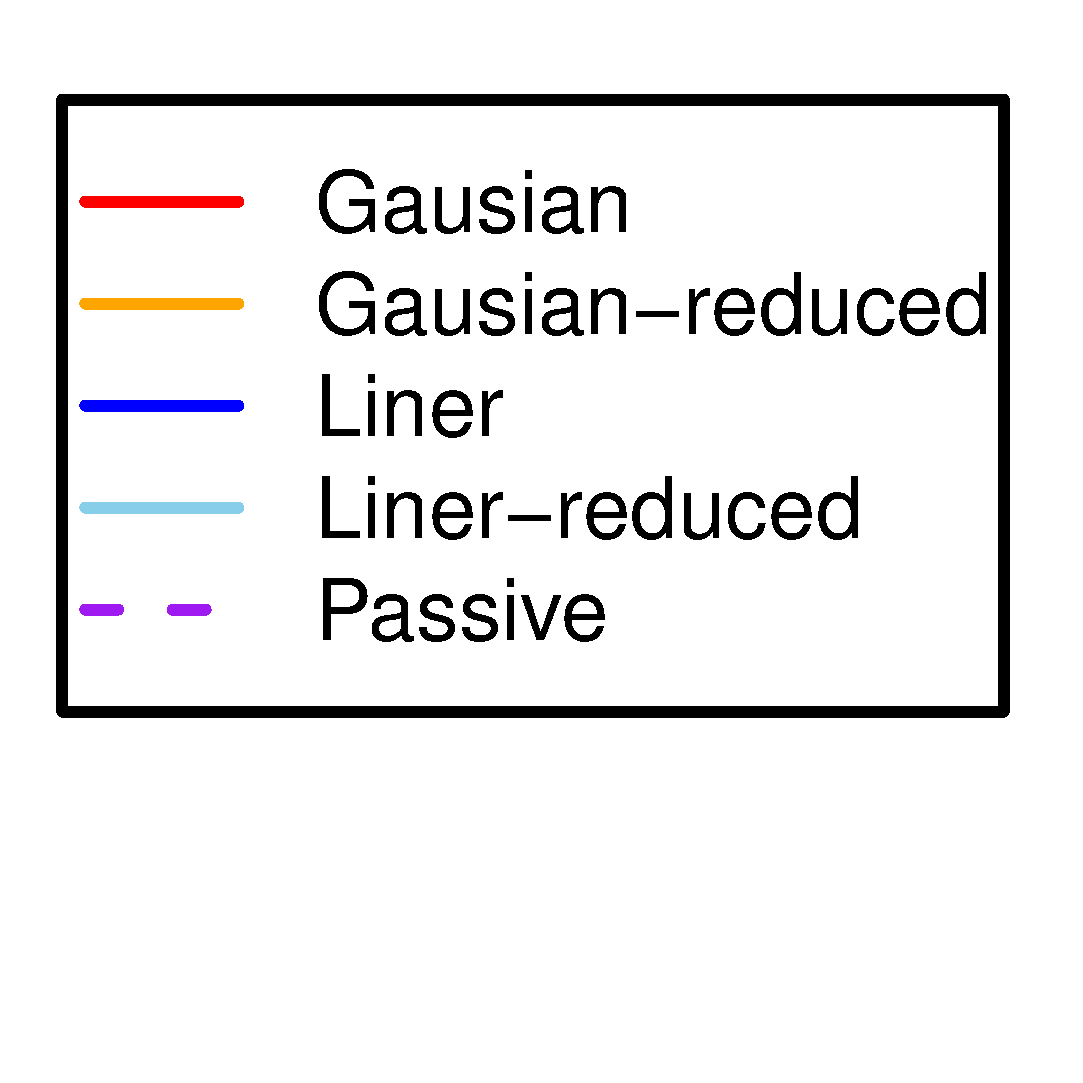
\includegraphics[width=0.6\columnwidth]{./Images_Result/k_test_legend.eps} 
       \end{subfigure}
       \begin{subfigure}{0.5\columnwidth}
         \centering
         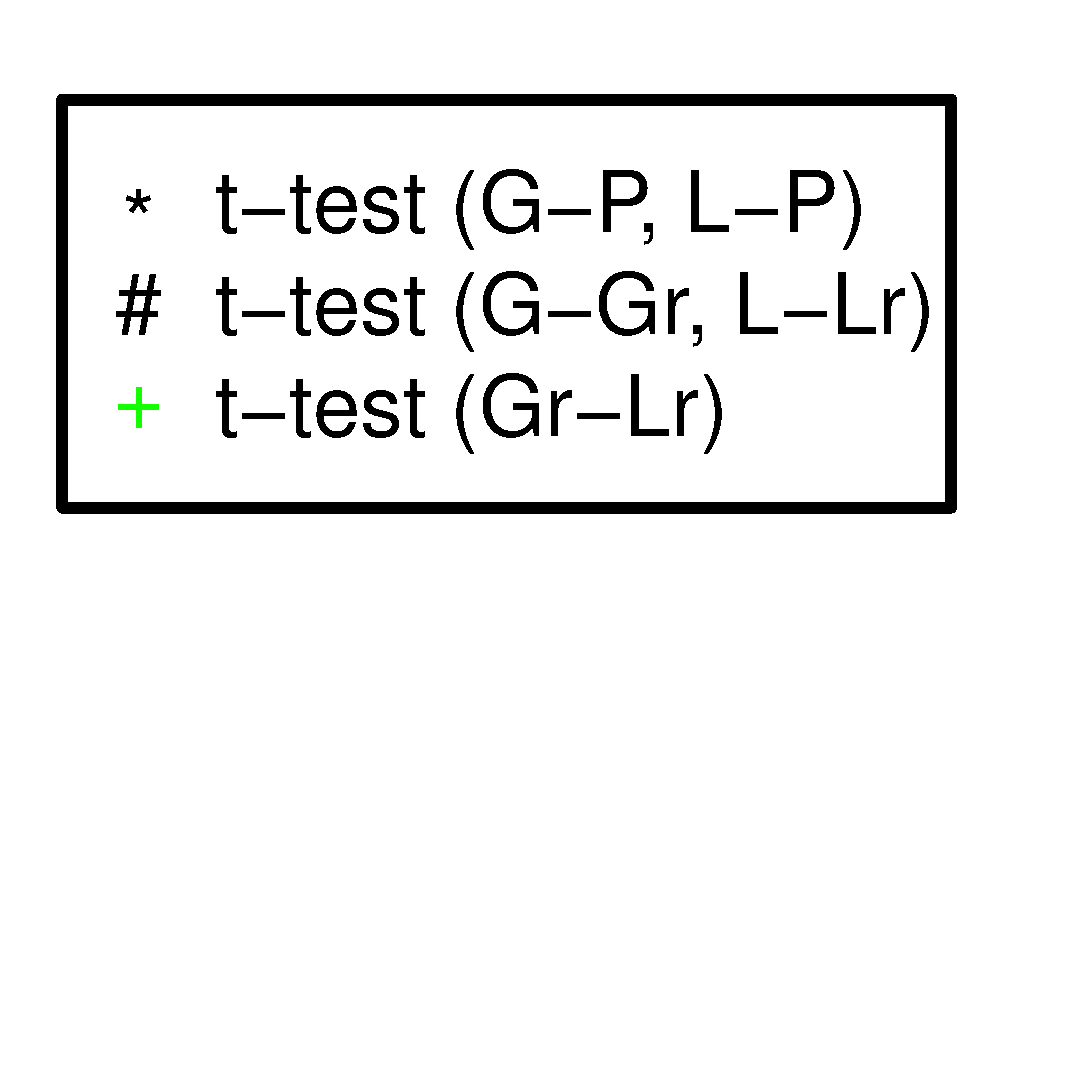
\includegraphics[width=0.6\columnwidth]{./Images_Result/test_legend.eps} 
       \end{subfigure}

       \vspace{-1.6cm}
       \caption{Ka$B%A%c%M%k$rF3F~$7$?:]$N7k2L(B1} %$B%Z!<%8%l%$%"%&%H$,7hDj$7$F$+$iHyD4@0$9$k(B
       \label{Ka_Result1}
     \end{figure}

   \vspace{-0.5cm}
     \begin{figure}[H]
       \begin{subfigure}{0.5\columnwidth}
         \centering
         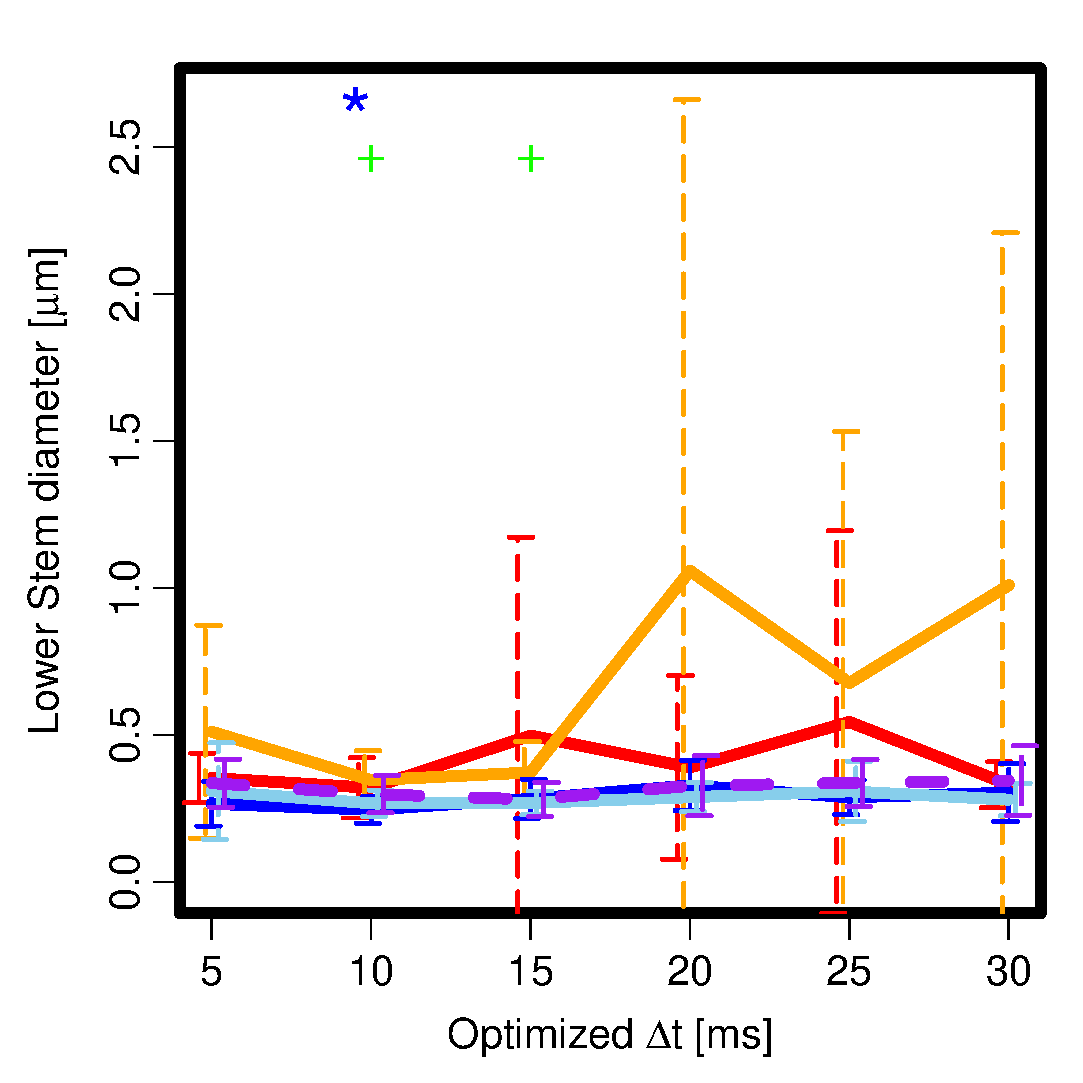
\includegraphics[width=0.8\columnwidth]{./Images_Result/k_test_Lower_Diam.eps} 
         \caption{Lower Dendrite$B$ND>7B(B}
         \label{k_Lower_Diam}
       \end{subfigure}
       \begin{subfigure}{0.5\columnwidth}
         \centering
         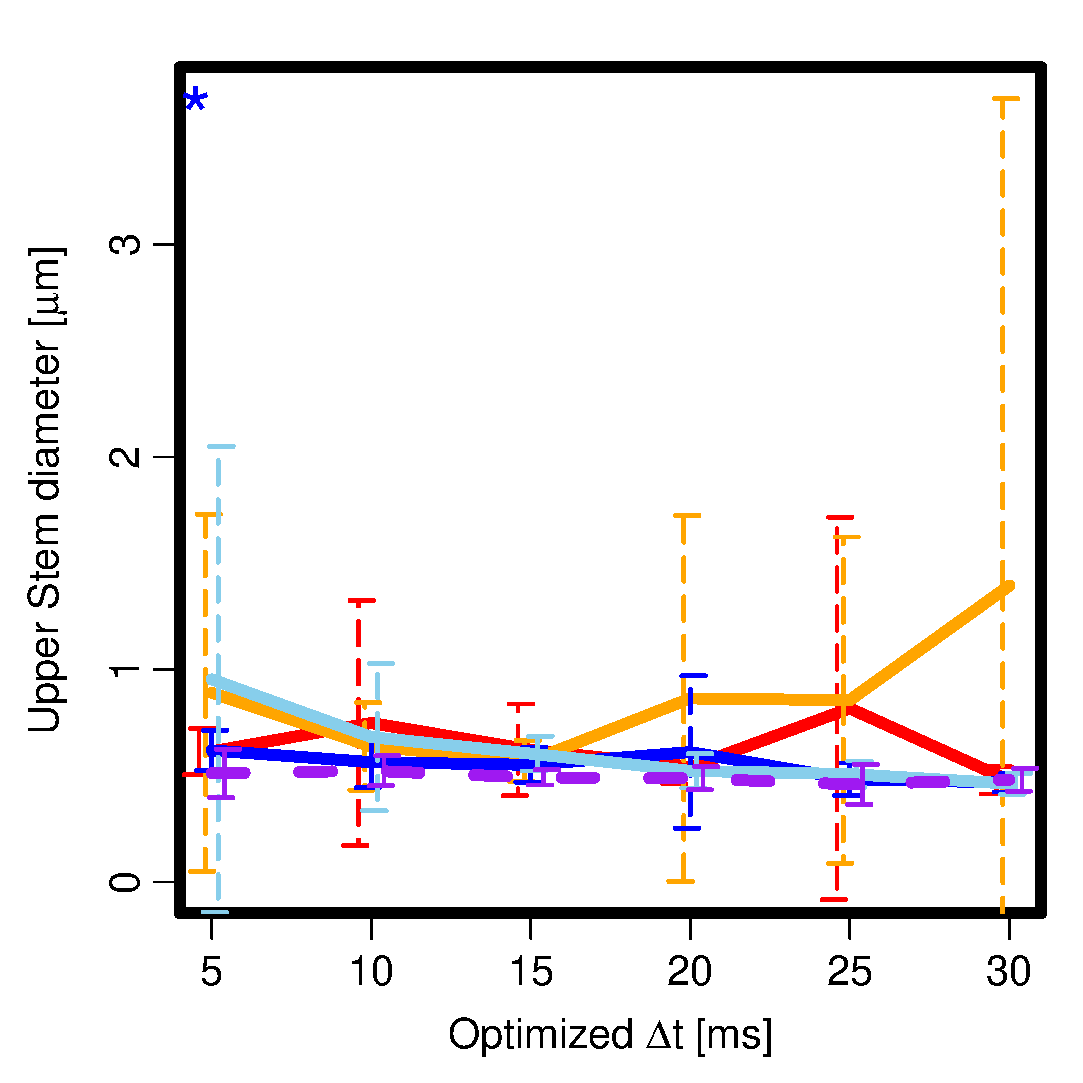
\includegraphics[width=0.8\columnwidth]{./Images_Result/k_test_Upper_Diam.eps}
         \caption{Upper Dendrite$B$ND>7B(B}
         \label{k_Upper_Diam}
       \end{subfigure}

       \begin{subfigure}{0.5\columnwidth}
         \centering
         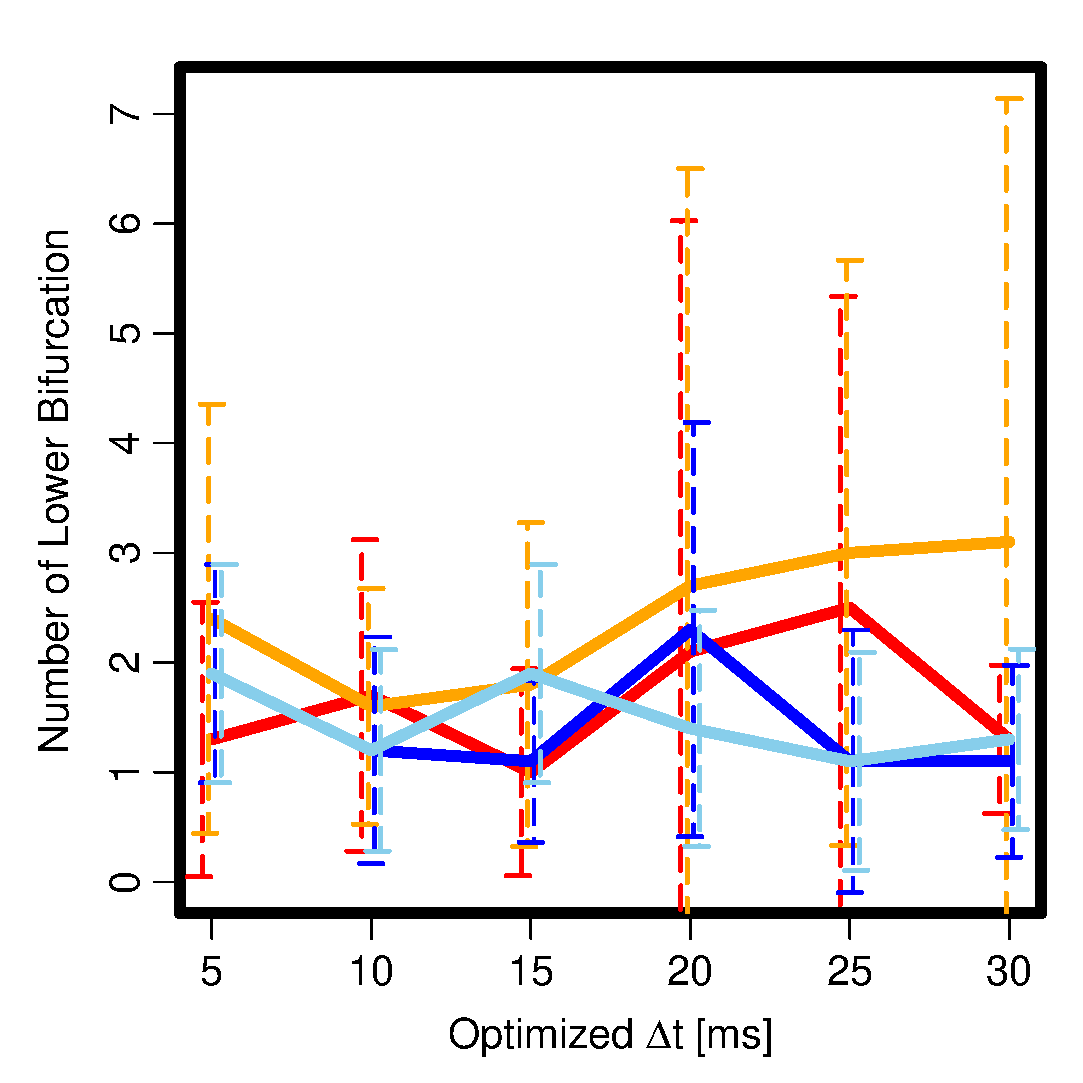
\includegraphics[width=0.8\columnwidth]{./Images_Result/k_test_N_Lower_bif.eps}
         \caption{Lower Dendrite$B$NJ,4t?t(B}
         \label{k_Lower_bif}
       \end{subfigure}
       \begin{subfigure}{0.5\columnwidth}
         \centering
         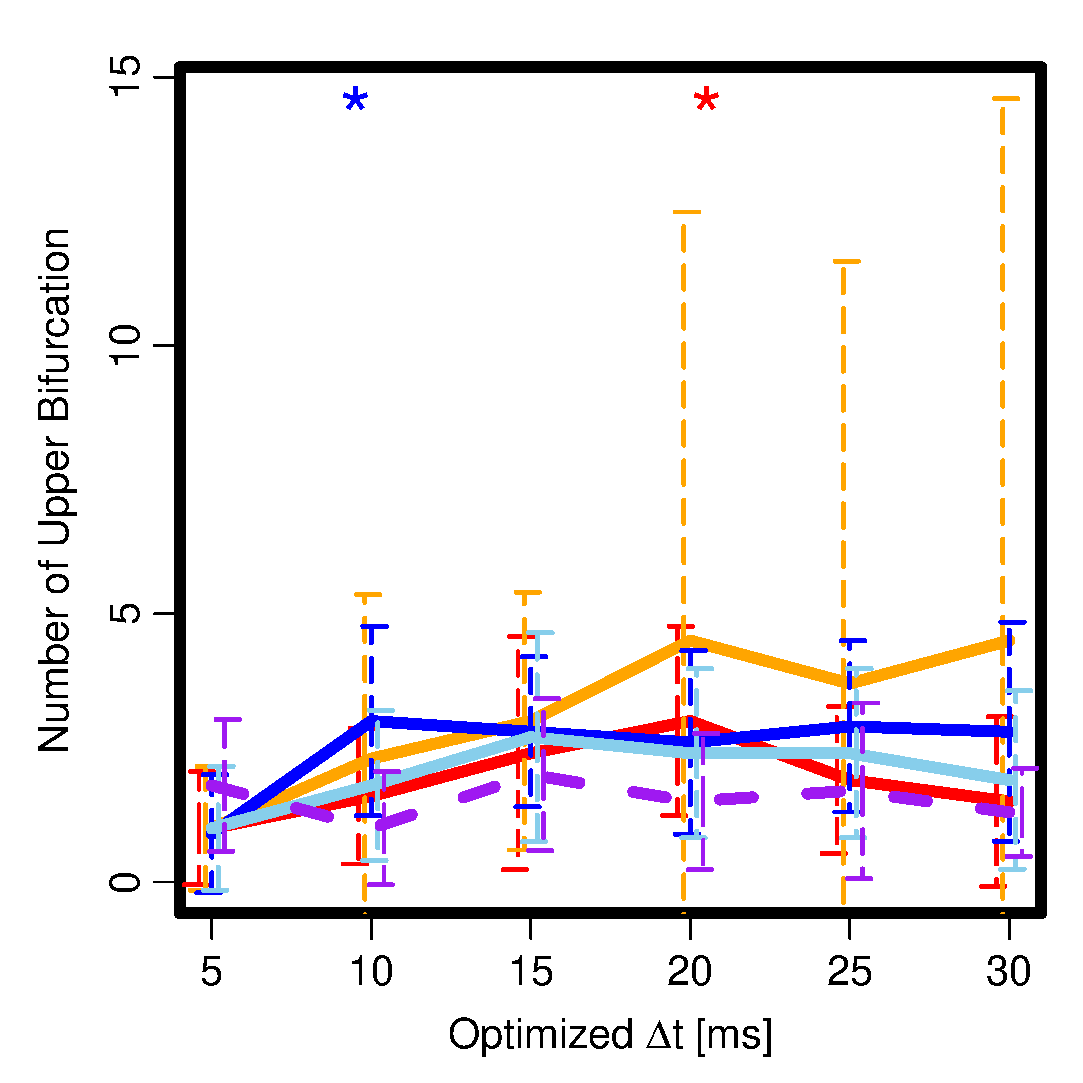
\includegraphics[width=0.8\columnwidth]{./Images_Result/k_test_N_Upper_bif.eps}
         \caption{Upper Dendrite$B$NJ,4t?t(B}
         \label{k_Upper_bif}
       \end{subfigure}

       \begin{subfigure}{0.5\columnwidth}
         \centering
         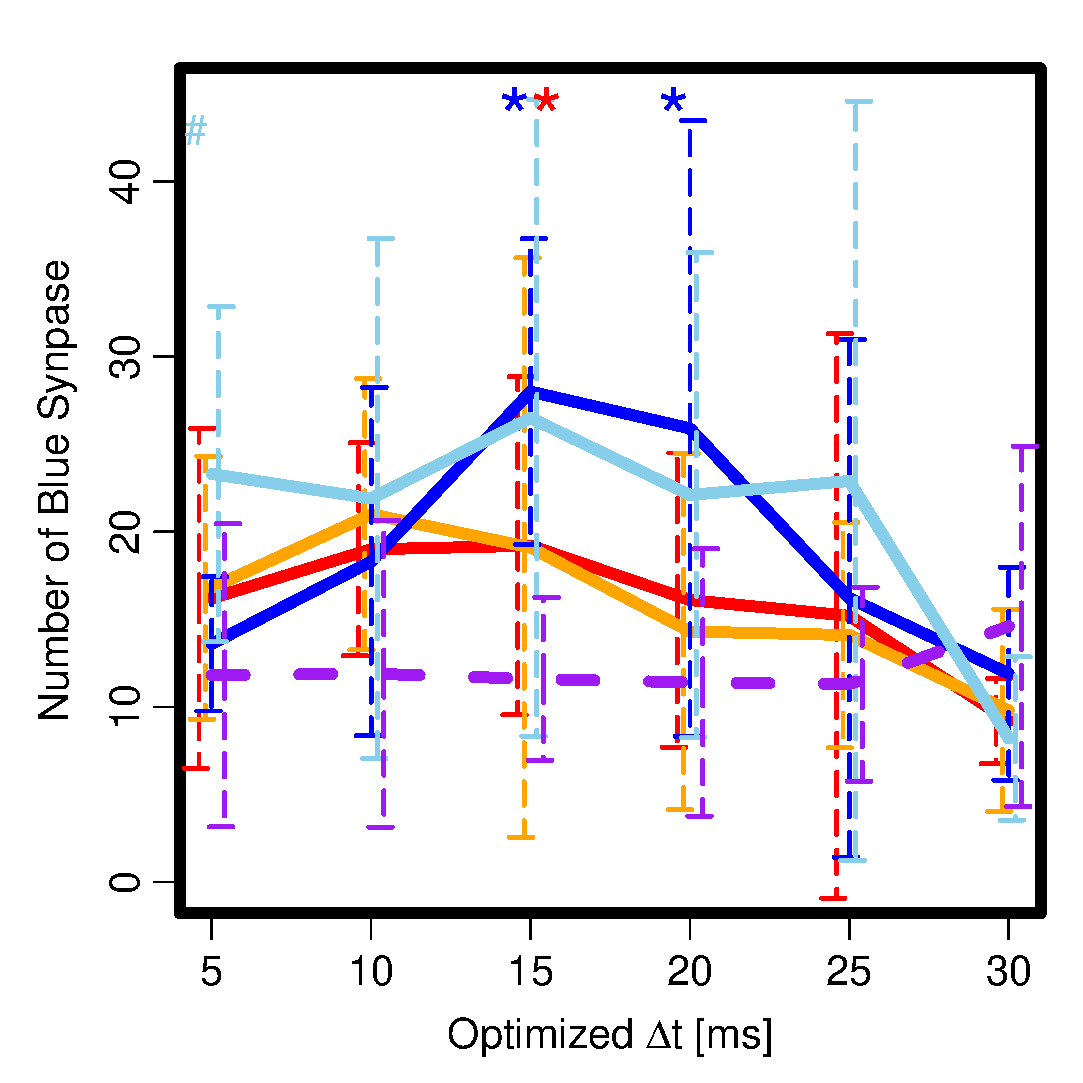
\includegraphics[width=0.8\columnwidth]{./Images_Result/k_test_N_Lower_Syn.eps}
         \caption{Lower Dendrite$B$N%7%J%W%9?t(B}
         \label{k_Lower_Syn}
       \end{subfigure}
       \begin{subfigure}{0.5\columnwidth}
         \centering
         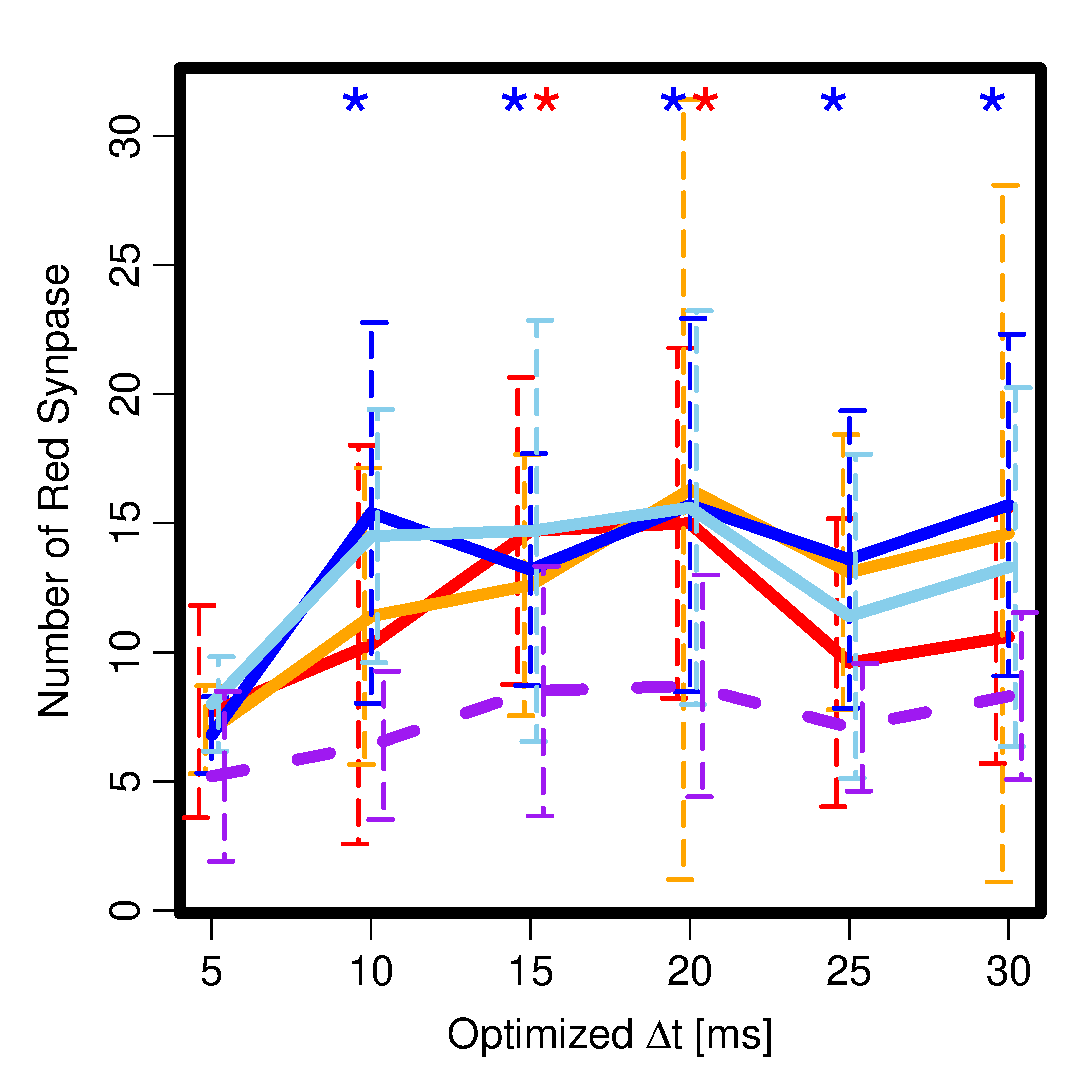
\includegraphics[width=0.8\columnwidth]{./Images_Result/k_test_N_Upper_Syn.eps}
         \caption{Upper Dendrite$B$N%7%J%W%9?t(B}
         \label{k_Upper_Syn}
       \end{subfigure}

       \vspace{-0.3cm}
       \begin{subfigure}{0.5\columnwidth}
         \centering
         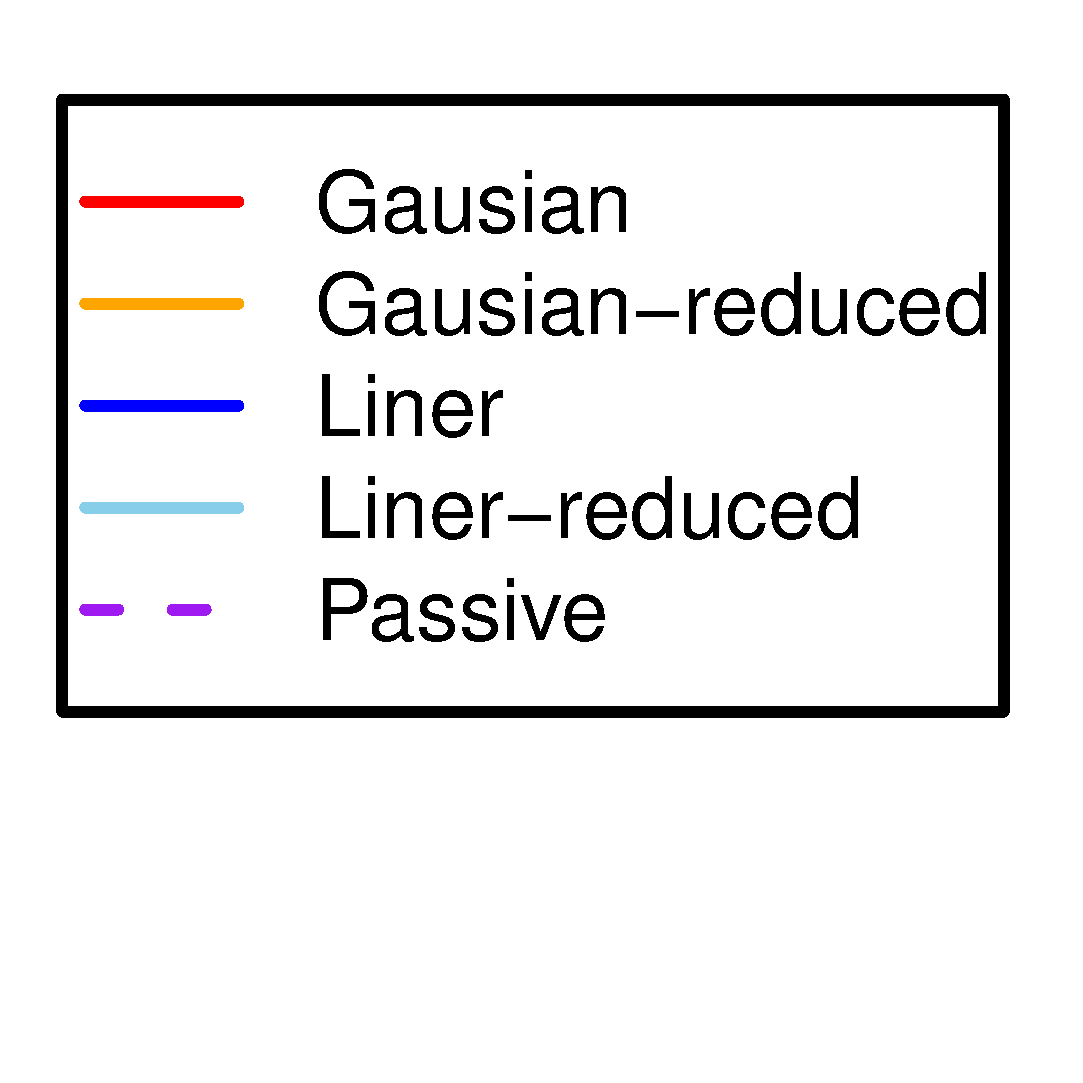
\includegraphics[width=0.6\columnwidth]{./Images_Result/k_test_legend.eps} 
       \end{subfigure}
       \begin{subfigure}{0.5\columnwidth}
         \centering
         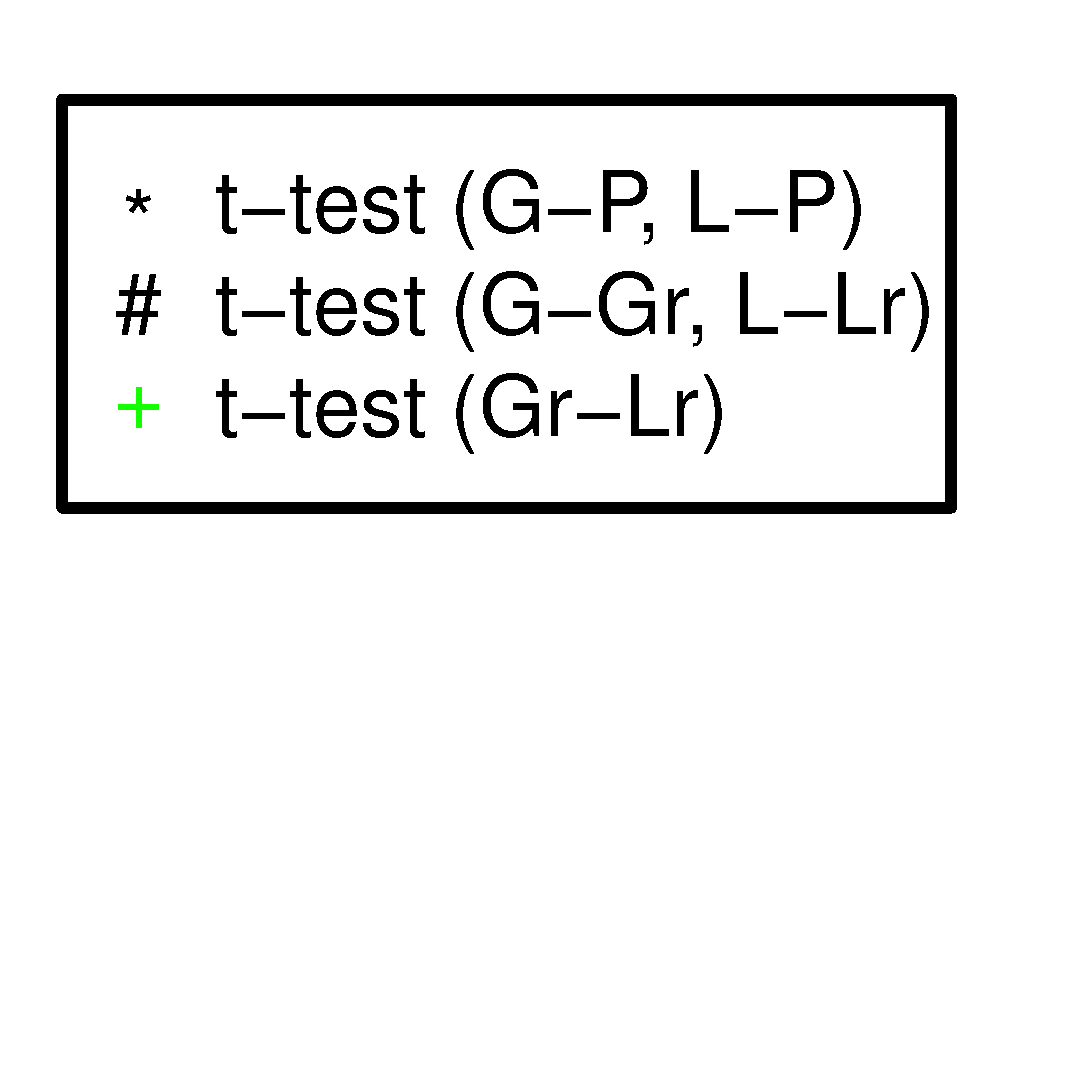
\includegraphics[width=0.6\columnwidth]{./Images_Result/test_legend.eps} 
       \end{subfigure}

       \vspace{-1.6cm}
       \caption{Ka$B%A%c%M%k$rF3F~$7$?:]$N7k2L(B2} %$B%Z!<%8%l%$%"%&%H$,7hDj$7$F$+$iHyD4@0$9$k(B
       \label{Ka_Result2}
     \end{figure}

  $B?^(B\ref{k_F}$B$h$j(BKa$B%3%s%@%/%?%s%9$rF3F~$7$?$3$H$G(BPassive$B$N>l9g$h$j$b(B$F$$BCM$,A}2C$7$F$$$k(B
  $B$3$H$,$o$+$k(B. $B@h9T8&5f$G$O(B${\Delta}t=5$[ms]$B$N$H$-$K:G$b9b$$(B$F$$BCM$,F@$i$l$F$$$?$,(B,
  $B$=$l$H$O0[$J$k7k2L$H$J$C$?(B. 
  $B?^(B\ref{k_TREE_K_ratio}$B$h$j8DBNI>2A$K$F%3%s%@%/%?%s%9NL$r9MN8$9$k>l9g$G$b?@7P:YK&(Bs
  $B$N(BKa$B%3%s%@%/%?%s%94^M-N($O$"$^$jJQ2=$,$J$$$3$H$,$o$+$k(B.

  $B?^(B\ref{Ka_V}$B$O(BKa$B%3%s%@%/%?%s%9$rF3F~$7$?:]$N%7%_%e%l!<%7%g%s$N0lNc$G$"$k(B. 
  $B<B@~$,(BKa$B%3%s%@%/%?%s%9$rF3F~$7$?%b%G%k$NKlEE0LGH7A$G$"$j(B, 
  $BGK@~$O$=$N?@7P:YK&$+$i(BKa$B%A%c%M%k$rIT3h@-2=(B($\overline{g}_{Ka} = 0$)$B$7$?>l9g$NKlEE0L$O7W$G$"$k(B. 
  $B?^(B\ref{Ka_V}$B$+$i$o$+$k$h$&$K(BKa$B%3%s%@%/%?%s%9$rF3F~$9$k$H(B, $B:YK&BN$G$NC&J,6K$O>.$5$/$J$k(B.

  \vspace{-0.5cm}
  \begin{figure}[H]
    \begin{subfigure}{0.6\columnwidth}
      \centering
      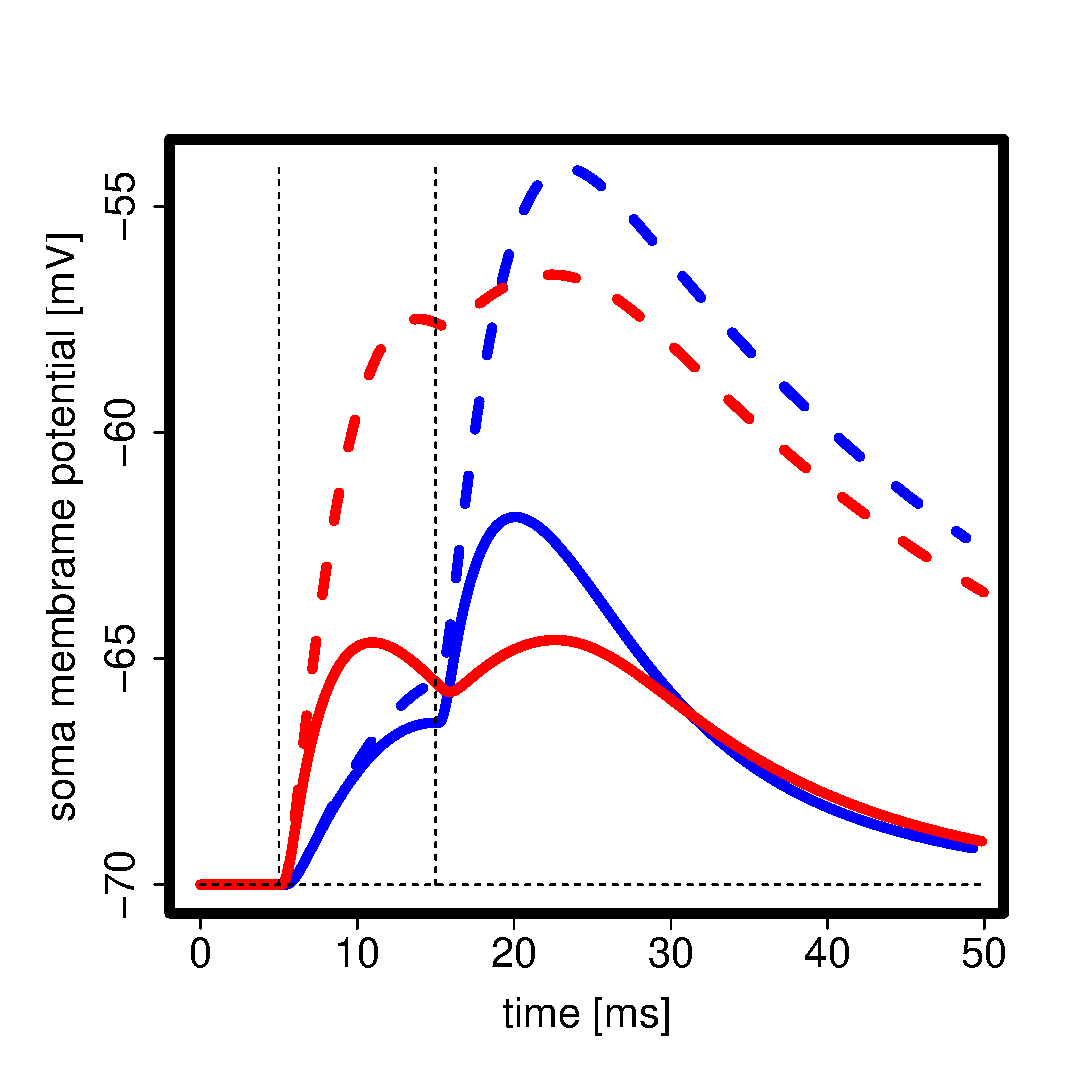
\includegraphics[width=0.7\columnwidth]{./Images_Result/k_V_dt10_C5.eps}
    \end{subfigure}
    \begin{subfigure}{0.5\columnwidth}
      \centering
      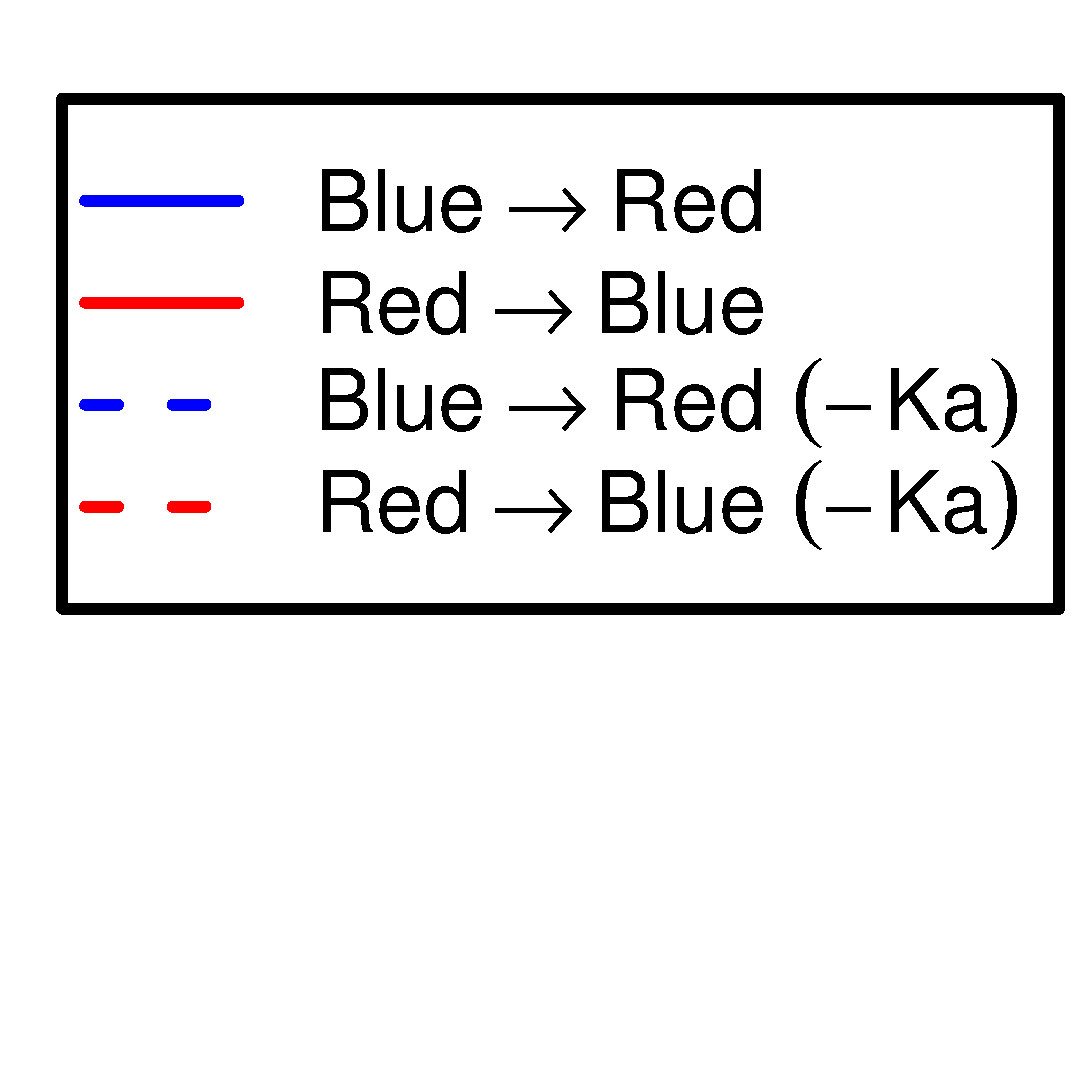
\includegraphics[width=0.6\columnwidth]{./Images_Result/k_2simulation_legend.eps}
    \end{subfigure}
      \caption{Ka$B!!KlEE0LGH7ANc(B(${\Delta}t = 10$[ms])}
      \label{Ka_V}
  \end{figure}
  %% $B?^(B\ref{k_morphos}$B$K:n@.$7$??@7P:YK&$N7ABVNc$r<($9(B. 
     
  %% \begin{figure}[H]
  %%   \begin{subfigure}{0.5\columnwidth}
  %%     \centering
  %%     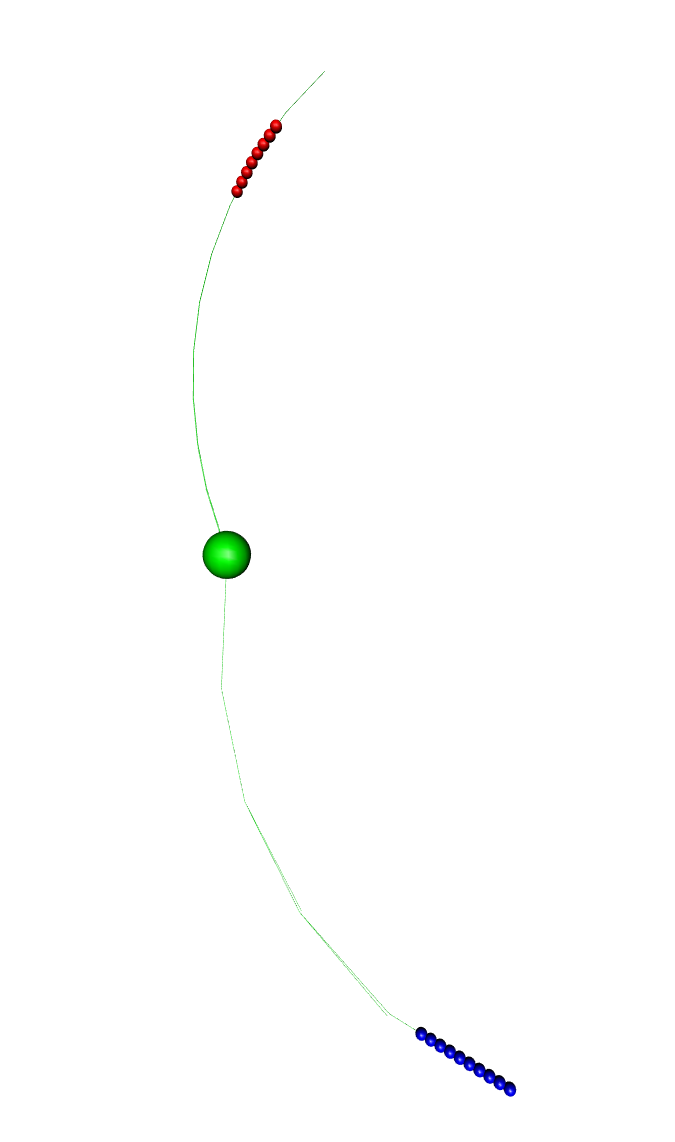
\includegraphics[width=0.5\columnwidth]{./Images_Result/k_liner_TREE_sample_dt5_C0.png} 
  %%     \caption{$B@~7AJ,I[(B}
  %%     \label{k_liner_morpho}
  %%   \end{subfigure}
  %%   \begin{subfigure}{0.5\columnwidth}
  %%     \centering
  %%     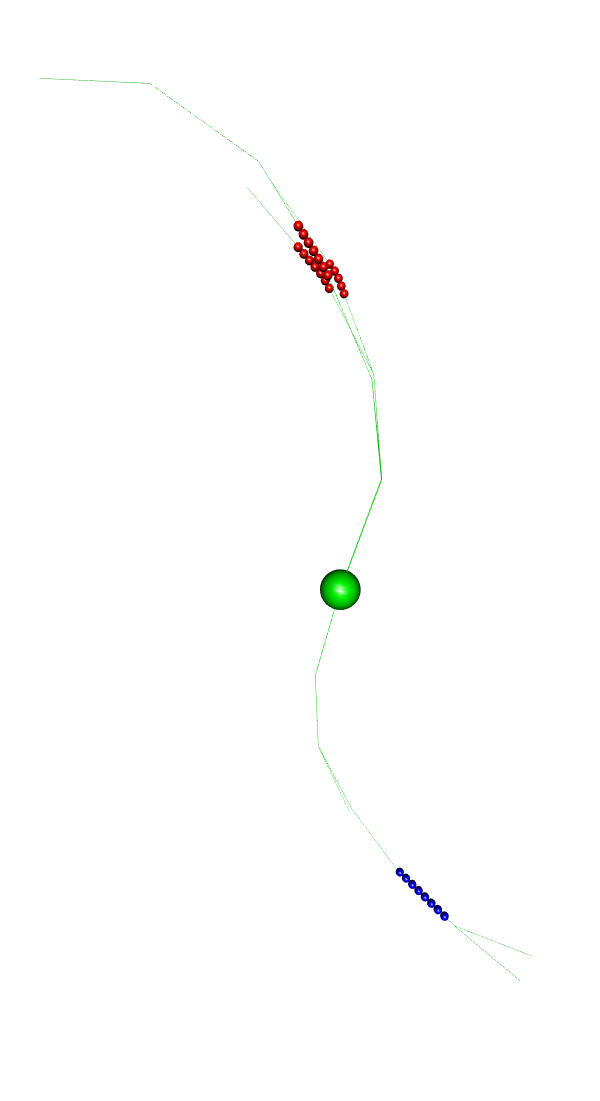
\includegraphics[width=0.5\columnwidth]{./Images_Result/k_gaus_TREE_sample_dt5_C0.png}
  %%     \caption{$B%,%&%9J,I[(B}
  %%     \label{k_gaus_morpho}
  %%   \end{subfigure}
  %%   \caption{Ka$B%3%s%@%/%?%s%9$rF3F~$7$??@7P:YK&$N7ABVNc(B}
  %%   \label{k_morphos}
  %% \end{figure}

%$B$3$l$OIUO?$K$7$?$[$&$,$h$5$=$&(B
   $B$^$?(B, $B?^(B\ref{k_Ka_dist_dt10}$B$K(B${\Delta}t = 10$[ms]$B$H$7$F:n@.$7$??@7P:YK&$N(B
   $B%3%s%@%/%?%s%9J,I[$r<($9(B.
   $B?^(B\ref{k_liner_dist_dt10}$B$O@~7AJ,I[$rMQ$$(B, $B?^(B\ref{k_gaus_dist_dt10}
   $B$O%,%&%9J,I[$rMQ$$$F$$$k(B. $B$^$??^(B\ref{k_liner_reduced_dist_dt10}$B$H(B
   $B?^(B\ref{k_gaus_reduced_dist_dt10}$B$O$=$l$>$l$N%3%s%@%/%?%s%9J,I[MM<0$G(B,
   $BI>2A<0$K$*$$$F%3%s%@%/%?%s%9$N9MN8$r9T$C$?>l9g$N7k2L$G$"$k(B. 
   \vspace{-0.5cm}
   \begin{figure}[H]
     \hspace*{-2cm}
     \begin{subfigure}{0.62\columnwidth}
       \centering
       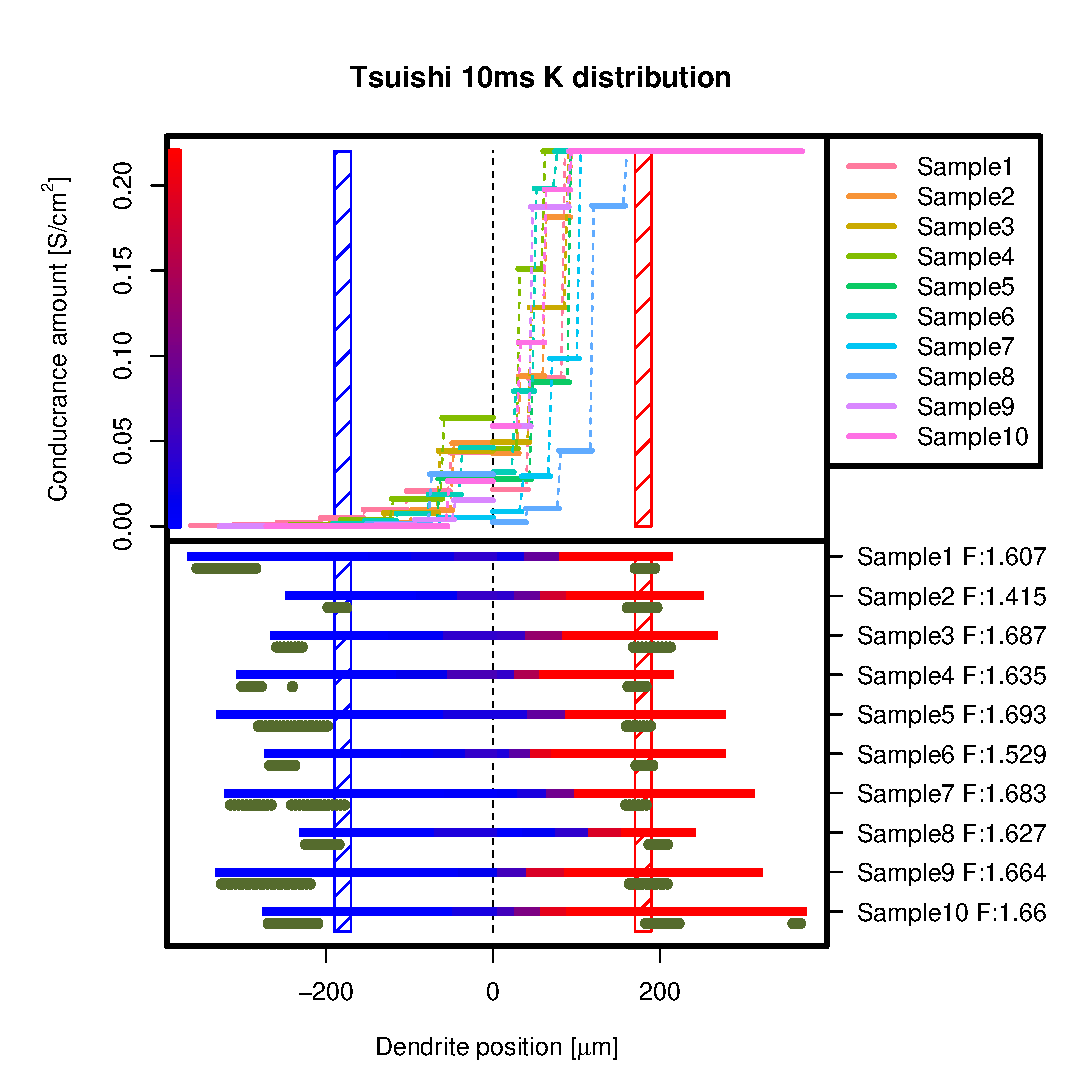
\includegraphics[width=\columnwidth]{./Images_Result/k_Rerative_liner_75_0_K_distribution_dt10.eps}
       \caption{$B@~7AJ,I[(B}
       \label{k_liner_dist_dt10}
     \end{subfigure}
     \begin{subfigure}{0.62\columnwidth}
       \centering
       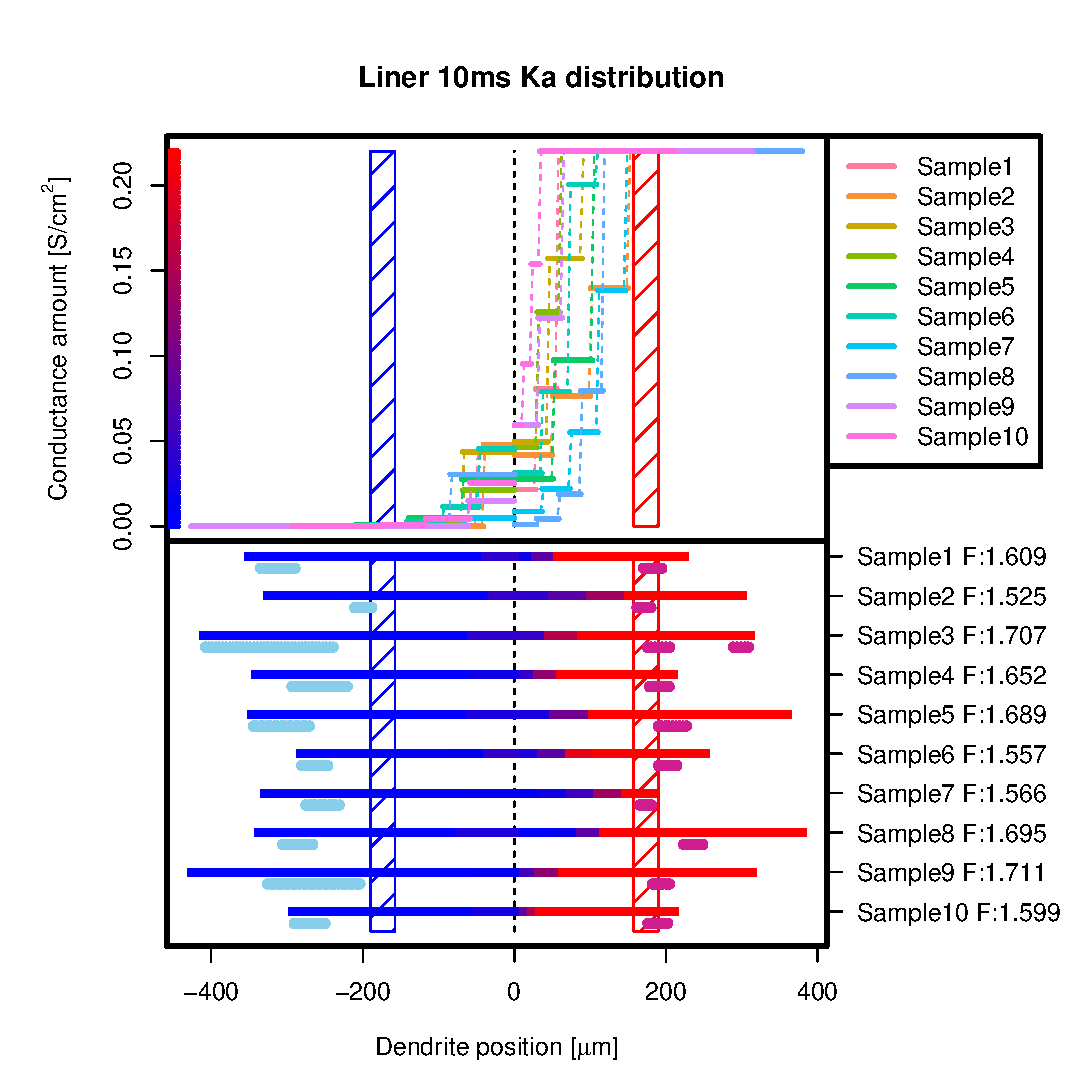
\includegraphics[width=\columnwidth]{./Images_Result/k_Rerative_liner_75_5_K_distribution_dt10.eps}
       \caption{$B@~7AJ,I[(B(reduced)}
       \label{k_liner_reduced_dist_dt10}
     \end{subfigure}

     \vspace{-1.5cm}
     \begin{subfigure}{\columnwidth}
       \centering
       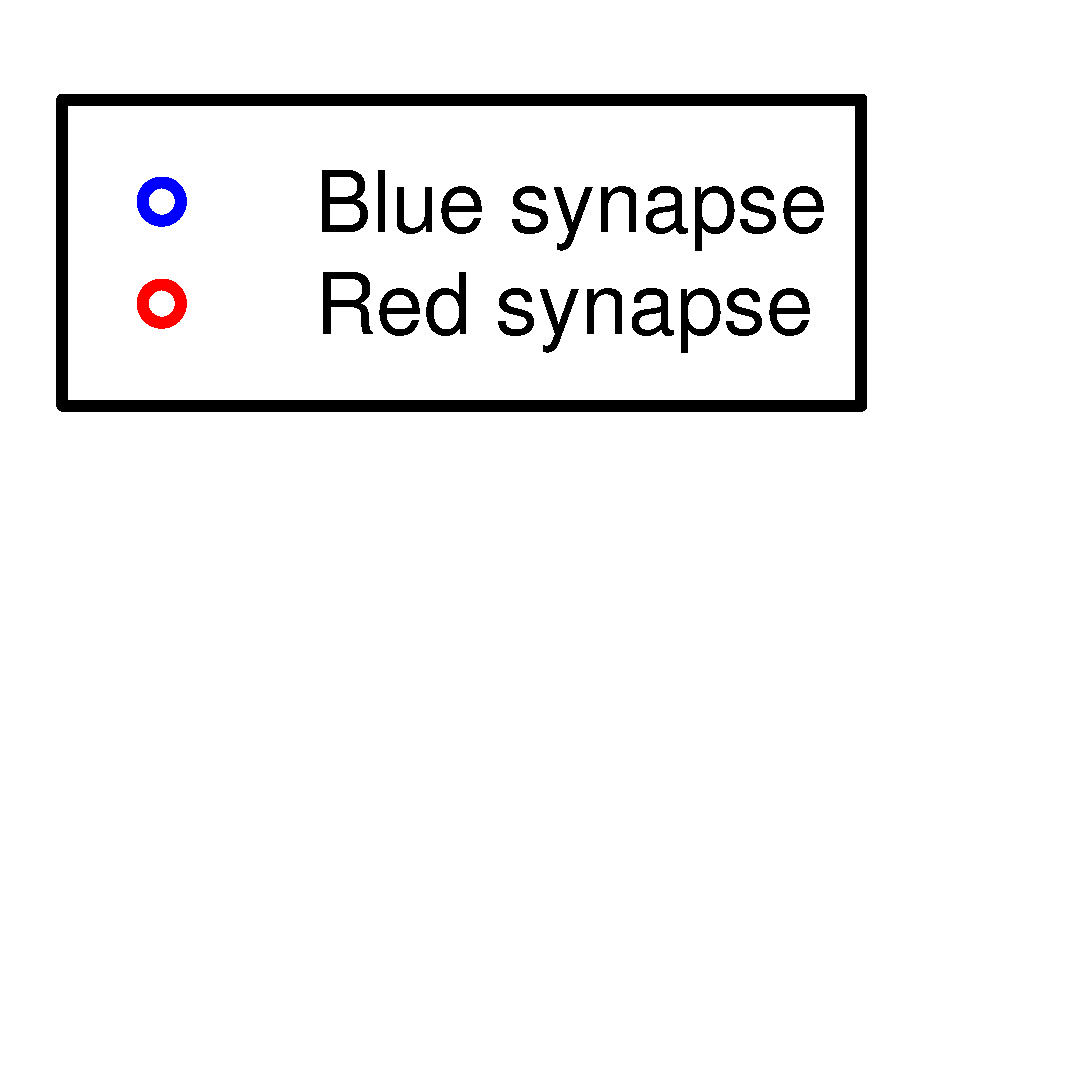
\includegraphics[width=0.35\columnwidth]{./Images_Result/Synapse_legend.eps} 
     \end{subfigure}
     \vspace{-4cm}

     \hspace*{-2cm}
     \begin{subfigure}{0.62\columnwidth}
       \centering
       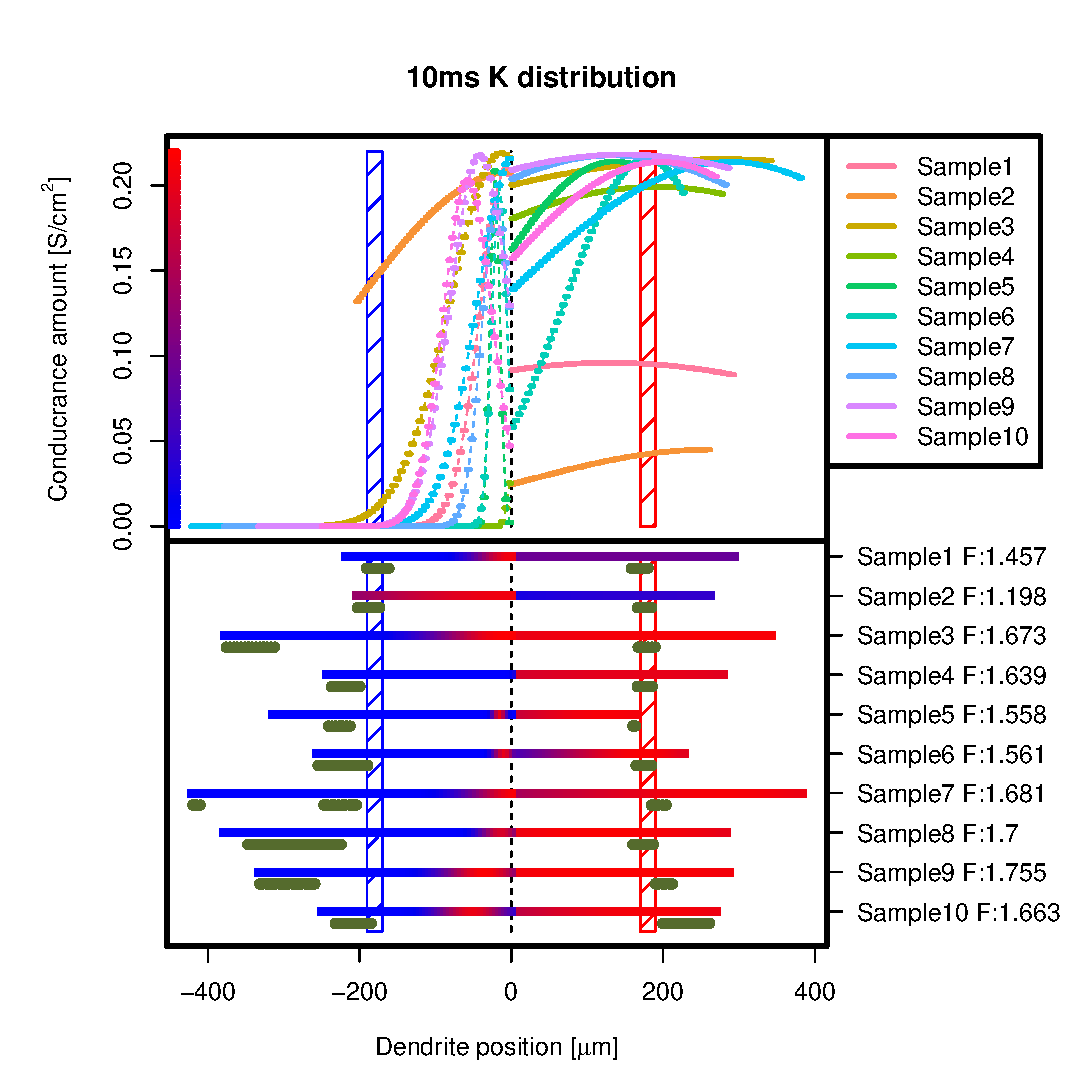
\includegraphics[width=\columnwidth]{./Images_Result/k_Rerative_Gaus_75_0_K_distribution_dt10.eps}
       \caption{$B%,%&%9J,I[(B}
       \label{k_gaus_dist_dt10}
     \end{subfigure}
     \begin{subfigure}{0.62\columnwidth}
       \centering
       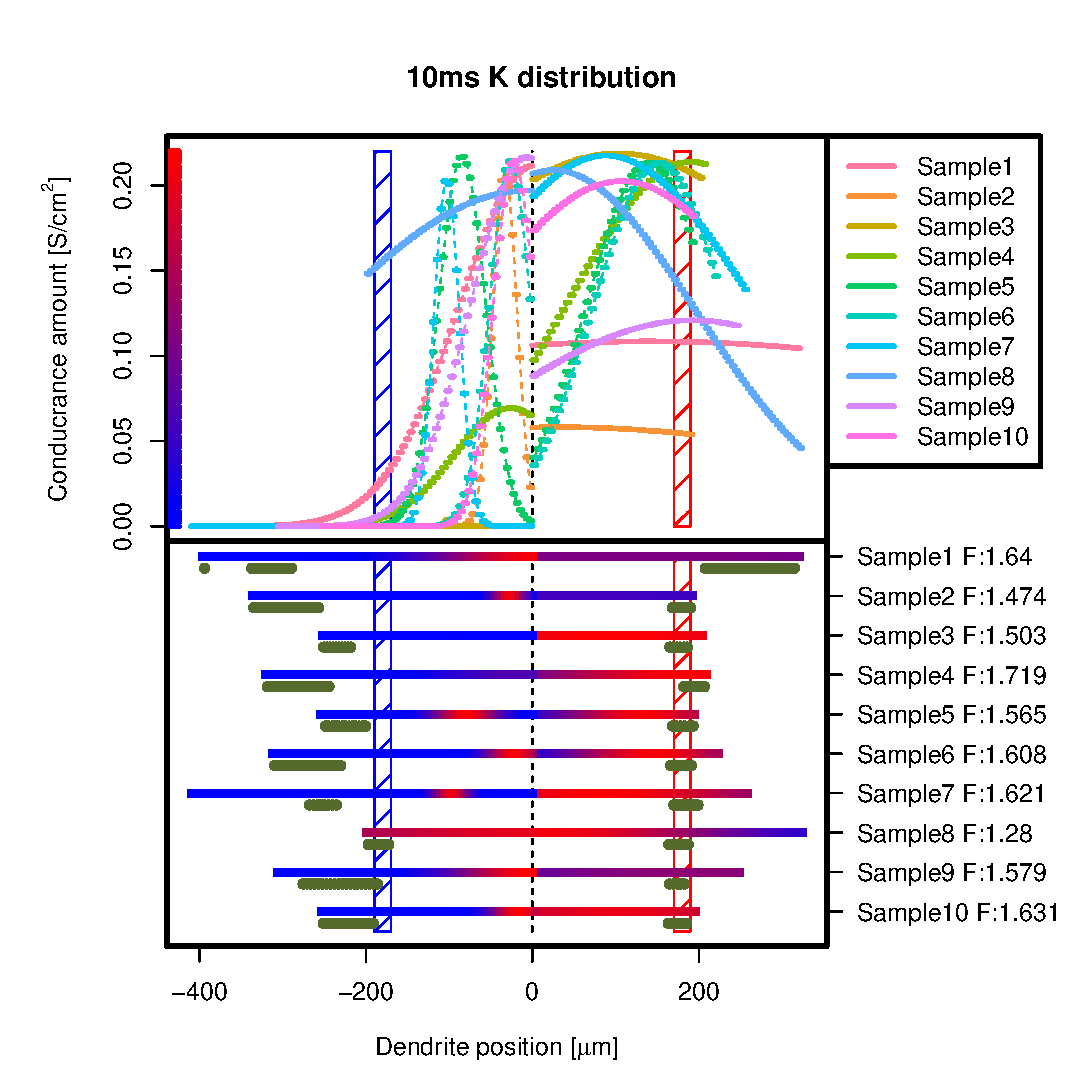
\includegraphics[width=\columnwidth]{./Images_Result/k_Rerative_Gaus_75_5_K_distribution_dt10.eps}
       \caption{$B%,%&%9J,I[(B(reduced)}
       \label{k_gaus_reduced_dist_dt10}
     \end{subfigure}
     
     \caption{${\Delta}t = 10$[ms]$B$G$N(BKa$B%3%s%@%/%?%s%9J,I[(B}
     \label{k_Ka_dist_dt10}
      \end{figure}

      \begin{figure}[H]
     \hspace*{-2cm}
     \begin{subfigure}{0.62\columnwidth}
       \centering
       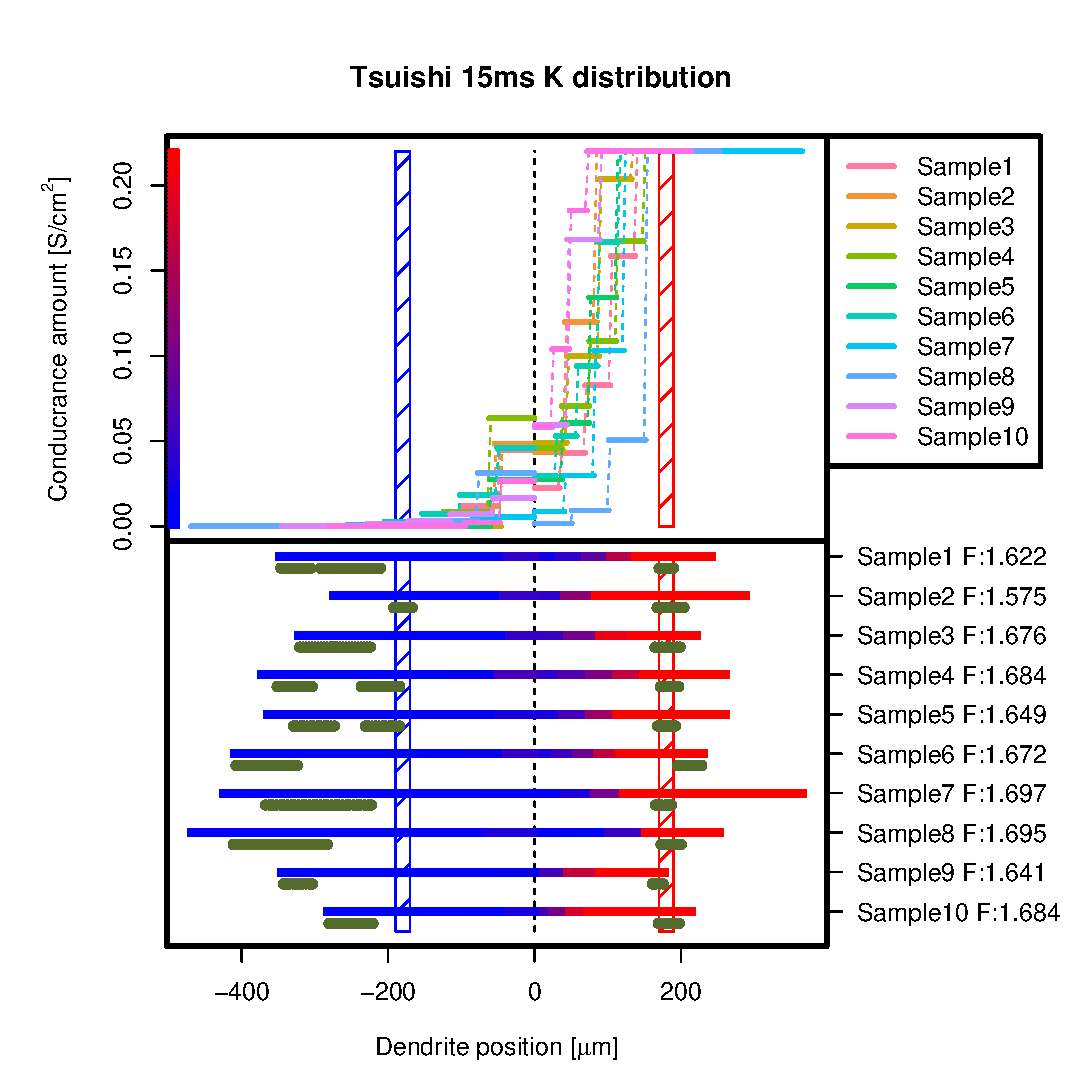
\includegraphics[width=\columnwidth]{./Images_Result/k_Rerative_liner_75_0_K_distribution_dt15.eps}
       \caption{$B@~7AJ,I[(B}
       \label{k_liner_dist_dt15}
     \end{subfigure}
     \begin{subfigure}{0.62\columnwidth}
       \centering
       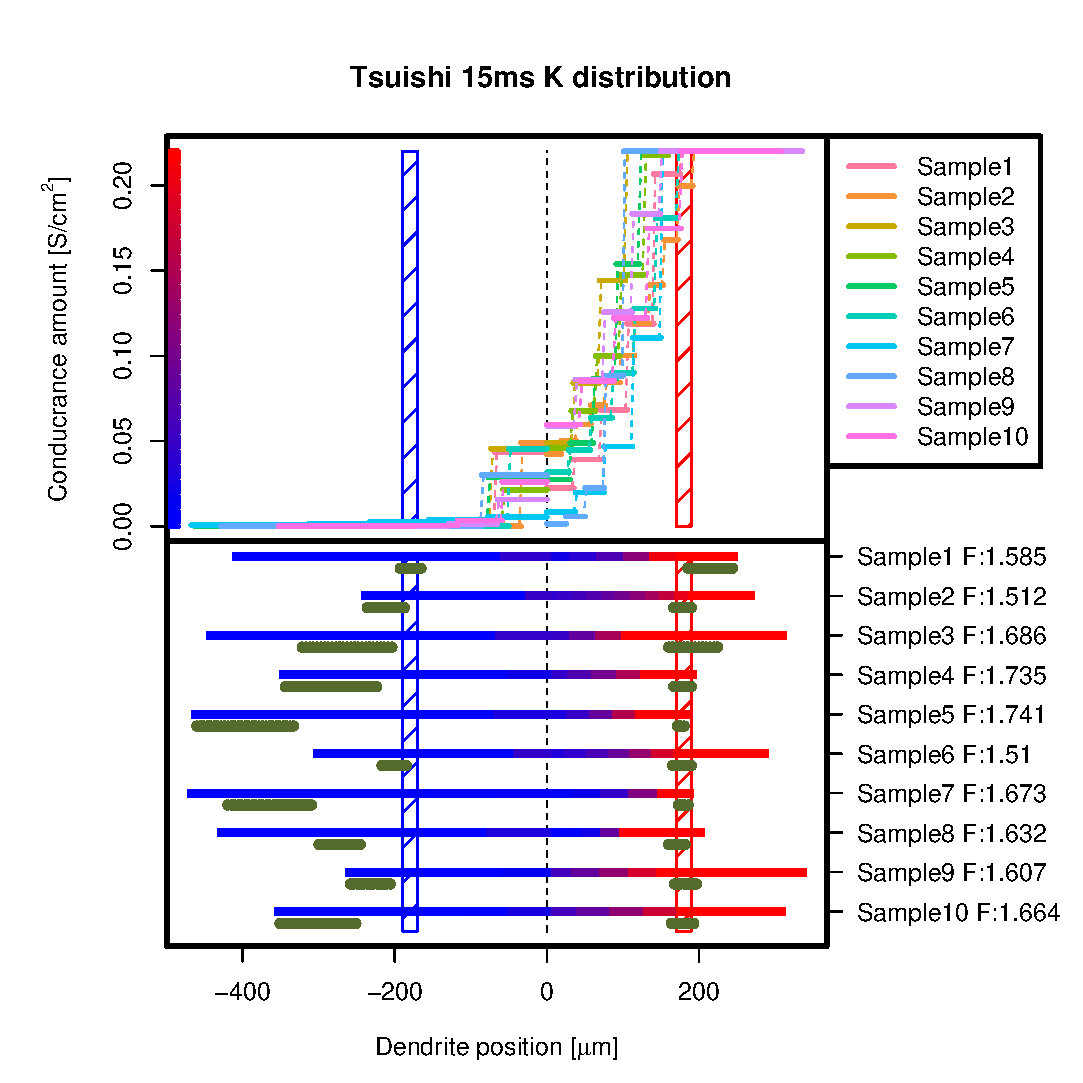
\includegraphics[width=\columnwidth]{./Images_Result/k_Rerative_liner_75_5_K_distribution_dt15.eps}
       \caption{$B@~7AJ,I[(B(reduced)}
       \label{k_liner_reduced_dist_dt15}
     \end{subfigure}

     \vspace{-1.5cm}
     \begin{subfigure}{\columnwidth}
       \centering
       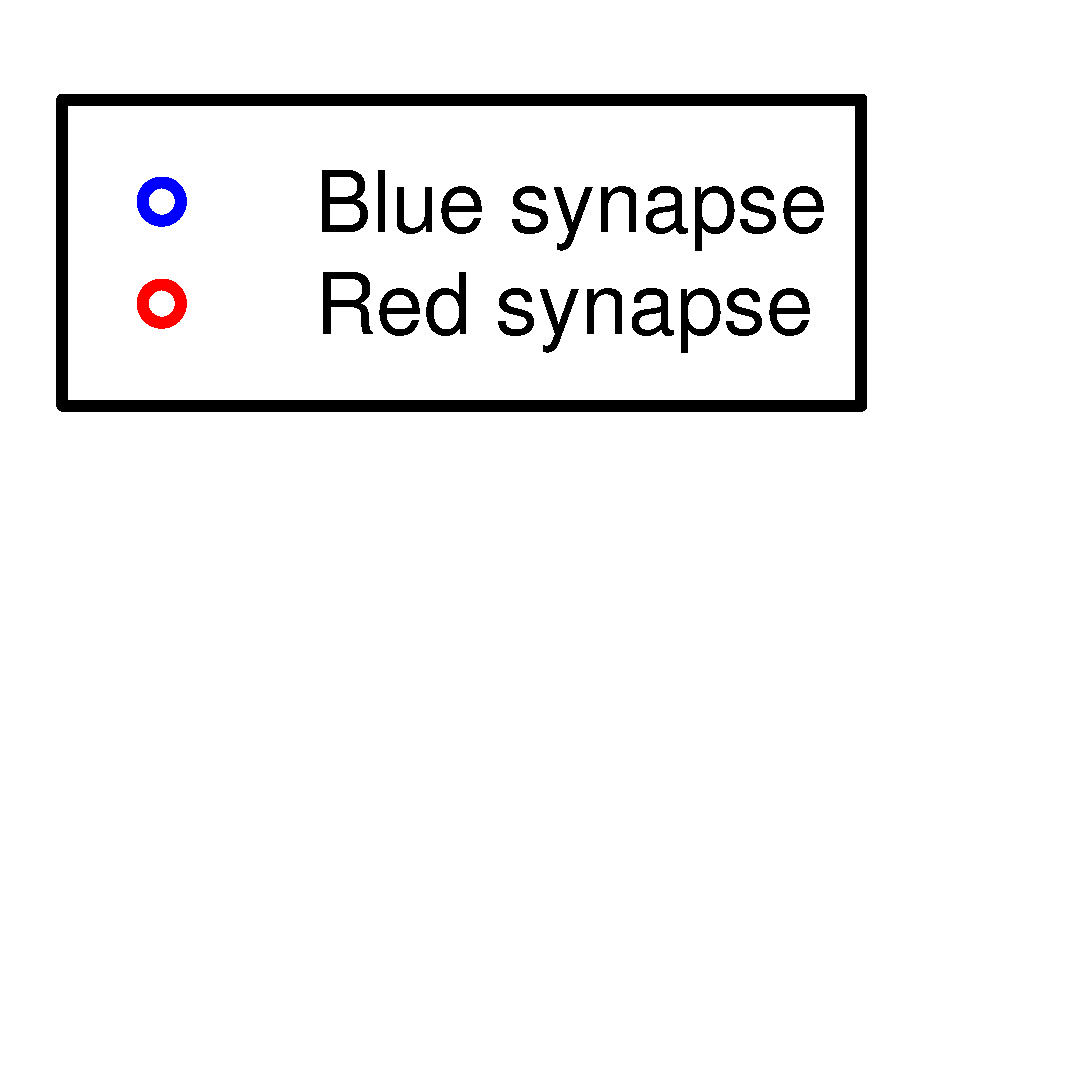
\includegraphics[width=0.35\columnwidth]{./Images_Result/Synapse_legend.eps} 
     \end{subfigure}
     \vspace{-4cm}

     \hspace*{-2cm}
     \begin{subfigure}{0.62\columnwidth}
       \centering
       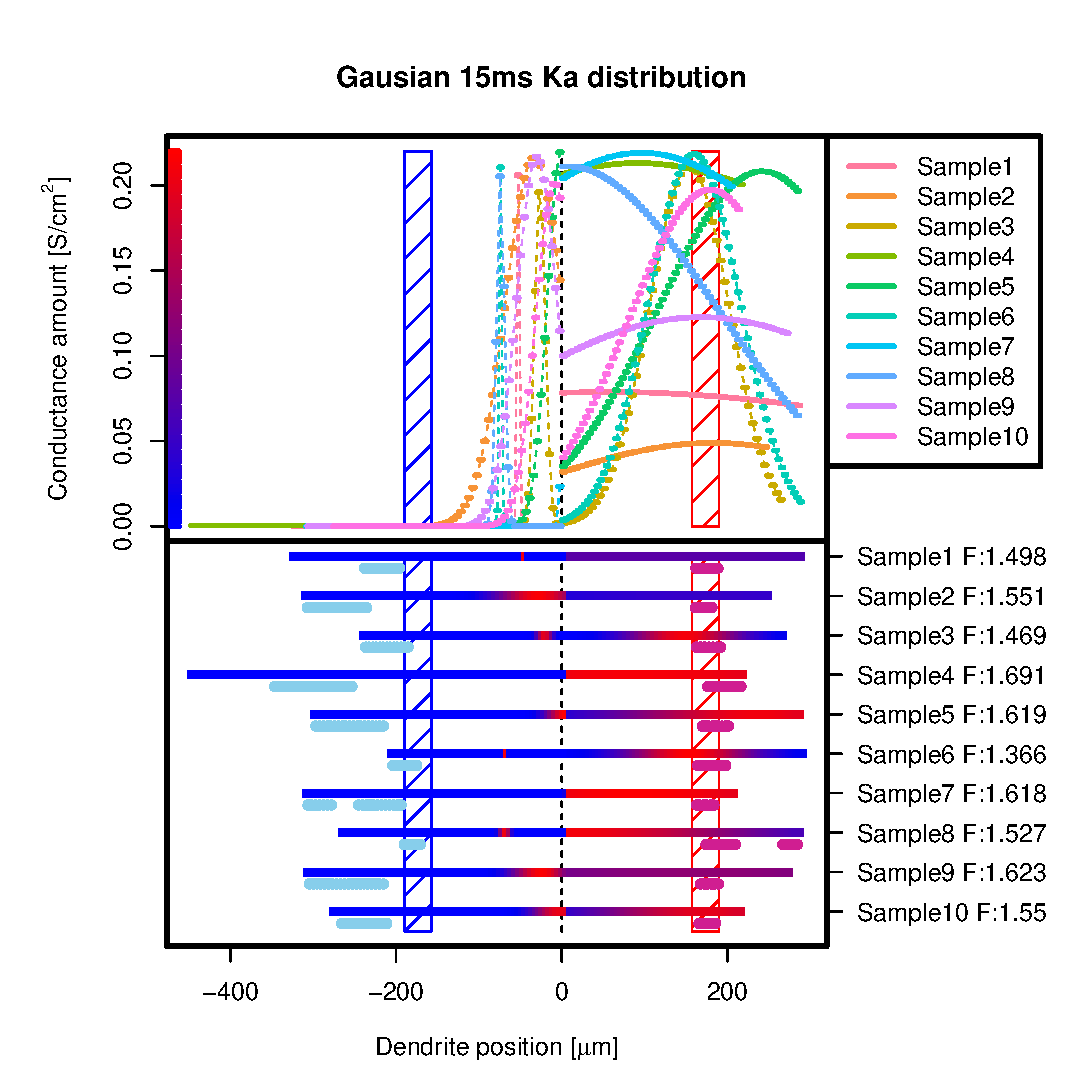
\includegraphics[width=\columnwidth]{./Images_Result/k_Rerative_Gaus_75_0_K_distribution_dt15.eps}
       \caption{$B%,%&%9J,I[(B}
       \label{k_gaus_dist_dt5}
     \end{subfigure}
     \begin{subfigure}{0.62\columnwidth}
       \centering
       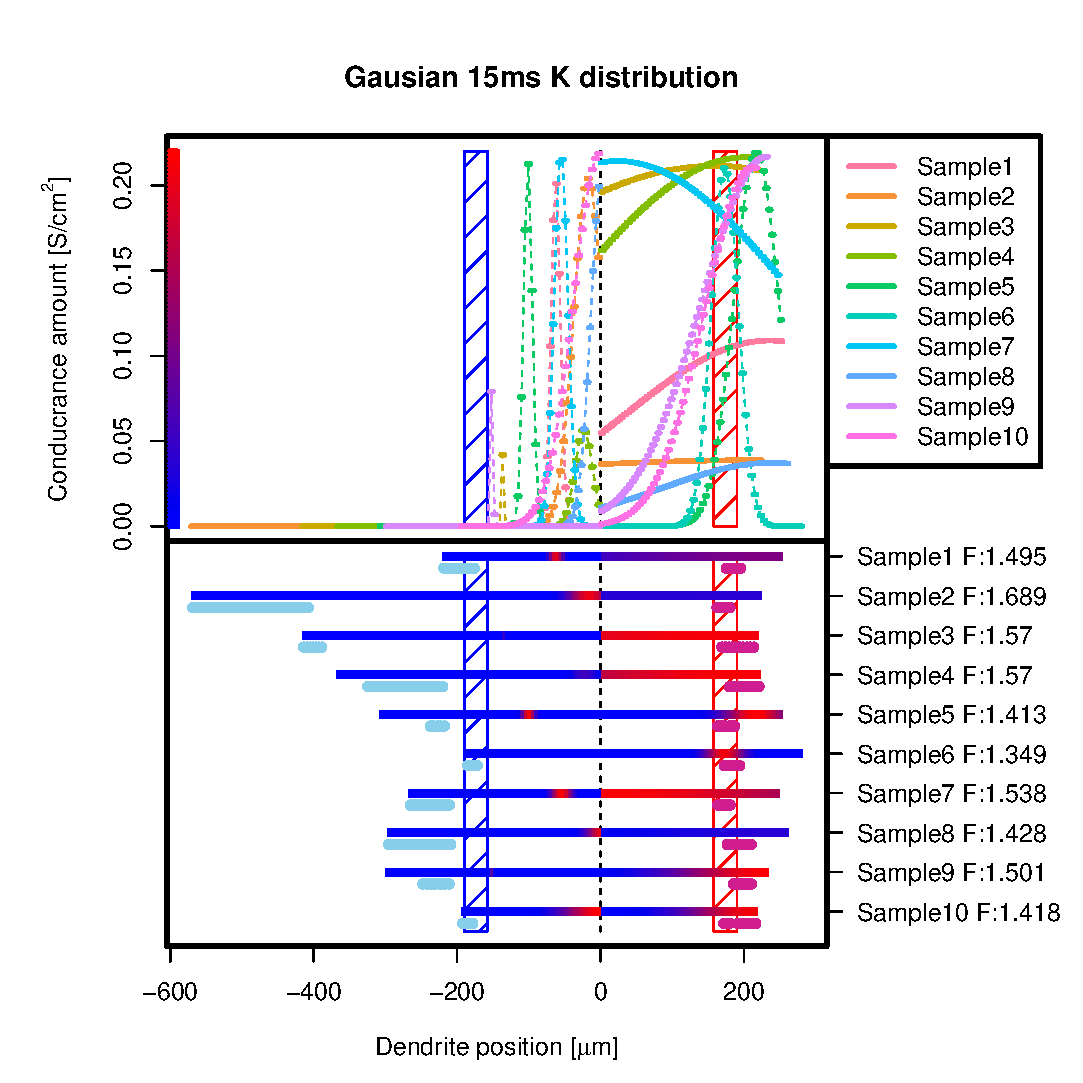
\includegraphics[width=\columnwidth]{./Images_Result/k_Rerative_Gaus_75_5_K_distribution_dt15.eps}
       \caption{$B%,%&%9J,I[(B(reduced)}
       \label{k_gaus_reduced_dist_dt15}
     \end{subfigure}
     
     \caption{${\Delta}t = 15$[ms]$B$G$N(BKa$B%3%s%@%/%?%s%9J,I[(B}
     \label{k_Ka_dist_dt15}
   \end{figure}

   $B?^(B\ref{k_gaus_reduced_dist_dt15}, $B?^(B\ref{k_upper_k_ratio}$B$+$i$o$+$k$h$&$K%,%&%9J,I[$rMQ$$$?>l9g(B
   $B$G$O(BUpper Dendrite$B$N:,85IU6a$G9b$$(BKa$B%3%s%@%/%?%s%9$NJ,I[$,8+$i$l$k(B.
